\documentclass[12pt]{report}
\usepackage{float}
\usepackage{graphicx}
\usepackage{wrapfig}
\usepackage{pythonhighlight}
\usepackage{svg}
\usepackage{hyperref}

\usepackage{listings}
\usepackage{color}
\definecolor{lightgray}{rgb}{.9,.9,.9}
\definecolor{darkgray}{rgb}{.4,.4,.4}
\definecolor{purple}{rgb}{0.65, 0.12, 0.82}
\graphicspath{ {/Users/andreaolivari/Dropbox/tesi/latex/img/} }

\lstdefinelanguage{javascript}{
  keywords={typeof, new, true, false, catch, function, return, null, catch, switch, var, if, in, while, do, else, case, break},
  keywordstyle=\color{blue}\bfseries,
  ndkeywords={class, export, boolean, throw, implements, import, this},
  ndkeywordstyle=\color{darkgray}\bfseries,
  identifierstyle=\color{black},
  sensitive=false,
  comment=[l]{//},
  morecomment=[s]{/*}{*/},
  commentstyle=\color{purple}\ttfamily,
  stringstyle=\color{red}\ttfamily,
  morestring=[b]',
  morestring=[b]"
}

\lstset{
   language=javascript,
   backgroundcolor=\color{white},
   extendedchars=true,
   basicstyle=\footnotesize\ttfamily,
   showstringspaces=false,
   showspaces=false,
   numbers=left,
   numberstyle=\footnotesize,
   numbersep=9pt,
   tabsize=2,
   breaklines=true,
   showtabs=false,
   captionpos=b
}


\title{\textbf{Security analysis of protocols used in IoT solutions}}
\author{Andrea Olivari}
\date{\today}

\begin{document}

\maketitle
\tableofcontents{}


\chapter{Introduction to IoT}
\bigskip
Internet of Things (IoT) is a neologism, introduced by Kevin Ashton~\cite{kevinashton} in 1999, which has become popular in recent years due to the growing interest from companies and because nowadays it is possible to produce small devices with a reasonable computational power.
Often, these small devices are embedded into bigger objects in order to improve them by making them, in some way, \emph{smart}.\\

IoT has a variety of different applications ranging from everyday things, like watches that measure how many kilometers we have walked during the day, to smart homes that control the air conditioning system on the basis of  temperature and pollution in the air, or even smart cities where semaphores adjust their times on traffic conditions.\\
But these are only three examples, IoT extends also to other fields like: health care, industrial monitoring, self driving cars and agriculture.\\

IoT is also changing the way software is developed: in order to produce good IoT systems, companies are brought to cooperate with each other,
moving from a one-company-does-it-all perspective to a let’s-work-together approach~\cite{successiot}.
This means that proprietary systems are no more a good choice and companies should embrace open systems in order to cooperate better.\\

From the financial point of view, IoT seems like a very profitable market: it is esteemed that the global IoT market will grow to \$457B by 2020~\cite{forbes}.\\ 
Assuming this forecast is on target, it means that lots of devices will be deployed in the network, exposing a device on the Internet also means exposing it to threats.\\
An interesting case of insecure IoT system is given by a luxury hotel in Austria \cite{whydoiot}: the electronic key system was attacked
by hackers that were able to lock out (or in, it depends) guests their rooms, until they paid a ransom; the system lacked a fundamental security
component necessary to avoid intrusion.\\
Long story short: after the attack, the hotel reverted to physical keys.\\
We can imagine other problematic situations that do not imply an attack; for instance: if a blackout occurs, is a guest still able to access his well paid room?\\
What if the content of the electronic key is not encrypted and it is possible to change its content in order to access other guests' room?\\
This event should also make us think if we really need an IoT system for every aspect of our life. An electronic key system is convenient, since you can configure the electronic key as you want in few seconds, but on the other hand it is also easy to corrupt its content, while it is not so simple to steal and duplicate a physical key.\\
 
The security aspect of an IoT application is not related only to possible external attacks by criminals but it also involves reliability; just think about a power plant monitored by an IoT system, if it is not well designed and for some reason it does not take the proper counter measures to an overload, a blackout can occur and the consequences are bad, mostly on the financial point of view.\\
These are the reasons why I am interested in analyzing the security aspect of IoT applications, considering that in near future
IoT could be integral part of our life I think it is crucial to develop secure system in order to avoid problems.


\section{Structure of an IoT application}
\bigskip
Most of times an IoT system is a large scale application that put in place different protocols, hardware and software.\newline
From the point of view of the protocols, there are lots of choices, such as: \emph{HTTP}, \emph{MQTT}, \emph{WebSocket}, \emph{ZigBee}, \emph{CoAP}, etc; each of them has its own advantages and disadvantages, so it is crucial to choose the one that fits our business logic; also considering that some protocols like MQTT or CoAP are used in sensors-server communication, while HTTP and WebSocket are used for client-server communications.\\

While dealing with IoT we can bump into different types of hardware: from constrained devices with low computational power to high performance cluster machines. Basically the ``dirty work" is taken from low power devices to the server, which elaborate received data or forward them to the cloud.\\
Talking about software, instead, we can work with a variety of programming languages: from a low level \emph{Assembly} to high level languages like \emph{C\#} or \emph{JavaScript}.\\

The development of an IoT system firstly requires a deep knowledge of the different parts of an application, hence the developement team should consist of experts with different skills and specializations.\newline
This little overview should help us to understand how difficult could be to design and develop an IoT application; Figure \ref{fig:iotstructure} illustrates the schema of a possible architecture of an IoT application.\\

\begin{figure}[H]
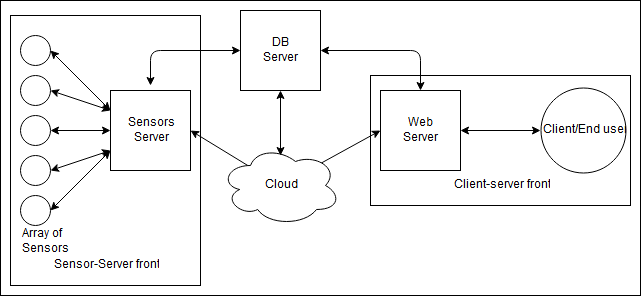
\includegraphics[width=13cm,height=12cm,keepaspectratio]{iotapp_architecture}
\caption{Possible structure of an IoT application}
\label{fig:iotstructure}
\end{figure}

\section{Structure of the thesis}
\bigskip
In this thesis I am going to analyze and discuss two of the most important and widespread IoT protocols: \emph{MQTT}, in part I, and \emph{ZigBee}, in part II.\\
More in details, we will start looking at their architecture and basic concepts, then we will discuss their security features, weaknesses and possible fixes.\\
Finally we list the best practices to follow in order to build a a secure communication environment.\\

With regard to the MQTT protocol, we discuss two interesting real use cases on which I had the opportunity to work during my internship, in order to see how much theory is respected in practice and how a real-world production system should be designed.\\

Unfortunately, I had not have the opportunity to work on industrial ZigBee projects, during my internship, since, as we will see, it is a protocol mainly aimed to home applications rather than industrial ones.\\\\

\part{MQTT}

\chapter{Protocol Overview}

\textsc{MQTT} \emph{(Message Queue Telemetry Transport)}~\cite{mqttrfc} is a simple, open and light-weight standarized messaging transport protocol, built on top of TCP/IP, invented by \emph{Andy Stanford-Clark} of \emph{IBM} and \emph{Arlen Nipper} of \emph{Cirrus Link Solutions}\cite{cirruslink} in 1999, with the following goals:

\begin{itemize}
\setlength{\itemindent}{+4mm}
  \item[$\bullet$] minimal battery loss
  \item[$\bullet$] minimal bandwidth usage
  \item[$\bullet$] simple to implement
  \item[$\bullet$] good quality delivery service
\end{itemize}\
All these aspects make this protocol particularly suitable for very constrained devices, which are often used in IoT services.\\\\
Nowadays MQTT is used in many different fields of applications:

 \begin{itemize}
 \setlength{\itemindent}{+4mm}
  \item[$\bullet$] Sensors communications \emph{(light, temperature, humidity, magnetic fields, pressure, intrusion detectors, etc})
  \item[$\bullet$] Health monitoring devices \emph{(e.g. blood pressure, insulin, heartbeat)}
  \item[$\bullet$] Fitness devices\emph{ (e.g. fitbit)}
  \item[$\bullet$] Location services
  \item[$\bullet$] Home automation kits used in \emph{smart homes}
  \item[$\bullet$] Inventory tracking \emph{(systems designed to track movements of inventory)}
  \item[$\bullet$] Automotive telematics
  \item[$\bullet$] Instant messagging applications \emph{(for instance, Facebook Messenger)}
\end{itemize}\

%\clearpage

%\section{Why is MQTT perfect for IoT?}
\bigskip
{\setlength{\parindent}{0cm}
Internet of Things requires a \emph{real-time event-driven communication model}, and it must be possible to send information in \emph{one-to-many} modality efficiently.\\
Since we mainly deal with sensors sending lots of data continuously, we need to reduce as much as possible the size of data packets to be sent, reliably.\\

HTTP is not suitable in this case because it is based on the request/reply paradigm and has a big network overhead. We must always remember that IoT deals with low-power devices whose connectivity can be really poor and extremely expensive.\\

MQTT is simple and light-weight, and can manage a huge number of communications as well as granting the delivery and reception of messages, without having to poll sensors.\\

%For all these reasons, \emph{Google Trends} highlights a strong and growing interest related to the keyword ``MQTT".
}


\section{Architecture and basic concepts}

%\subsection{Publish/Subscribe pattern}
\label{ssec:pubsubpattern}
\bigskip
MQTT protocol exploits the modern publish/subscribe pattern, sometimes called pub-sub, which is a valid alternative to the traditional client-server model, in which a client communicates directly with an endpoint.\\
This design pattern provides asynchronous communication between clients.\\
Nodes are arranged around a component, usually called \emph{broker} or \emph{dispatcher}, in a star topology and, as we can see in Figure~\ref{fig:mqttArchitecture}, they can talk to each other by publishing and subscribing to topics; we discuss them in the section \ref{ssec:topicsandsub}.

\begin{figure}[H]
\includegraphics[width=12cm,height=12cm,keepaspectratio]{mqtt_architecture1}
\caption{MQTT Architecture}
\label{fig:mqttArchitecture}
\end{figure}

The sender of a message is called \emph{publisher}, while who is interested in receiving it is called \emph{subscriber}.\\
So, a broker is nothing but a kind of message container, known by both the publisher and subscriber, able to filter all incoming messages and distribute them accordingly.\\

\subsection{Topics and subscription}
\label{ssec:topicsandsub}
\bigskip
Clients publish or subscribe to particular topics, which are simply message subjects having a syntax similar to file pathnames. For instance, assuming we want to name two topics related to sensors placed in our kitchen and bedroom, we may opt for the following names: $$'sensors/home/lights/kitchen'$$ $$'sensors/home/lights/bedroom'$$\\
MQTT brokers use these topics to decide to who forward the messages to.\\\\ 
It is important to notice that publishers and subscribers do not know about the existence of one another, but they can talk anyway.
This behaviour is part of a process called \emph{decoupling of publisher and subscriber}, which can be split in three dimensions:

\begin{itemize}
  \setlength{\itemindent}{+4mm}
  \item[$\bullet$] \emph{space decoupling}: publisher and subscriber do not know each other; to be more clear, they do not know the IP address and port used by the other one
  \item[$\bullet$] \emph{time decoupling}: publisher and subscriber do not have to be synchronized and may run at different times
  \item[$\bullet$] \emph{synchronization decoupling}: operations on both components are not suspended while publishing or receiving messages; they are independent
\end{itemize}\

Figure \ref{fig:pubsubschema} shows a schematic  example of the publish/subscribe pattern combined with topics subscription, but, in order to better understand it, let's keep a reference list of the existent MQTT messages we are going to deal with. Figure~\ref{fig:mqttmsgs} lists all of them.


\begin{figure}[H]
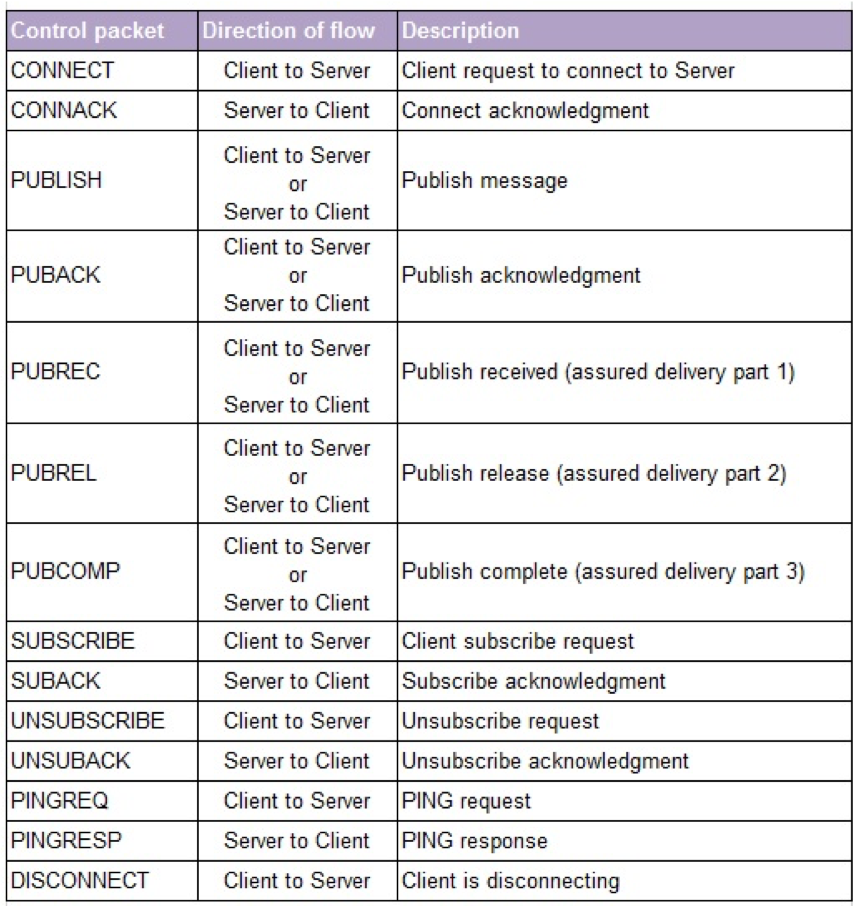
\includegraphics[width=14cm,height=14cm,keepaspectratio]{mqtt_messages}
\centering
\caption{MQTT messages}
\label{fig:mqttmsgs}
\end{figure}

Message types' names are self-explanatory, anyway we will describe some of them more in details along the way.\\\\
Now, let's analyze the example we were talking about.

\begin{figure}[H]
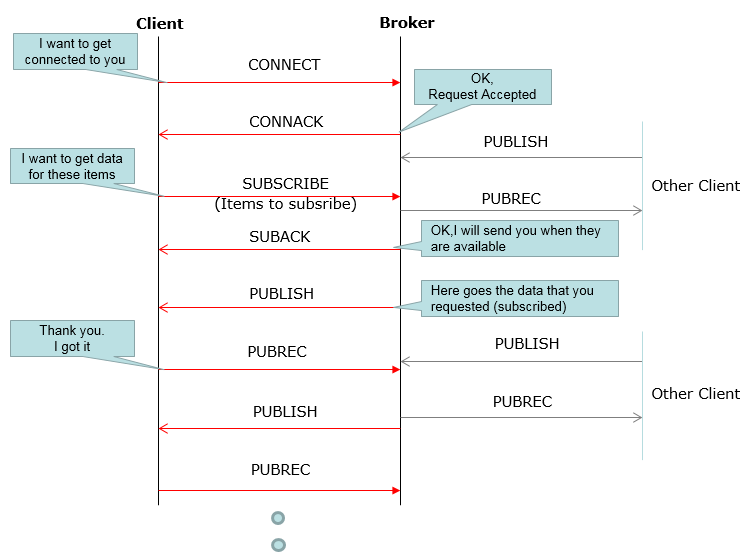
\includegraphics[width=12cm,height=11cm,keepaspectratio]{pubsub_schema1}
\centering
\caption{Publish/Subscribe combined with Topics}
\label{fig:pubsubschema}
\end{figure}

\begin{enumerate}
\setlength{\itemindent}{+5mm}
\item A client wants to connect to the broker, and sends the proper CONNECT packet, whose structure is visible in Figure \ref{fig:connectpacket}.

\begin{figure}[H]
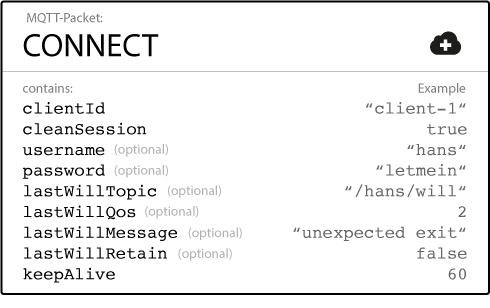
\includegraphics[width=7cm,height=7cm,keepaspectratio]{connect_message}
\centering
\caption{CONNECT packet}
\label{fig:connectpacket}
\end{figure}
where:

\begin{itemize}
\setlength{\itemindent}{+4mm}
\item[$\bullet$] \emph{clientId} is a identifier, unique per broker, each client must have.\\
  \emph{If you do not need a state to be held by the broker, in MQTT 3.1.1 it is possible to send an empty value.}
  \item[$\bullet$] \emph{clean session} is used to establish persistent connections
  \item[$\bullet$] \emph{username} and \emph{password} are used to authenticate the user in a password-protected broker. These credentials are sent in plain-text, we will see later how to face this issue.
  \item[$\bullet$] \emph{keep alive} is nothing but a time interval used by the client to commit regular \texttt{PING Request} messages to the broker (that will reply with a \texttt{PING Response} message)
\end{itemize}

\item Once the broker has received a connection request, it replies with a \texttt{CONNACK} packet, containing a field called \emph{return code}. 
This field can assume six different values, where the first one (Connection accepted) indicates the connection has been accepted, while the others indicate that connection has been refused for some reason (Unacceptable protocol version, Invalid identifier, Server unavailable, Not Authorized, Bad username and password).

\item Assuming that the connection has been accepted by the broker, then the client can choose to publish a message or subscribe to a topic.\\\\
In the first case it will send a \texttt{PUBLISH} packet, whose structure is visible in figure \ref{fig:publishpacket}.

\begin{figure}[H]
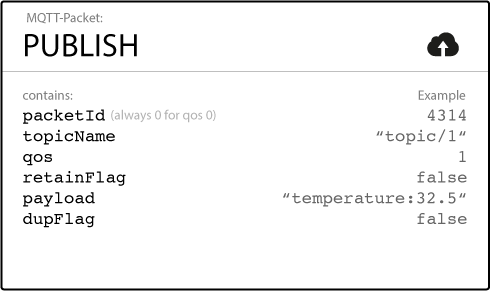
\includegraphics[width=7cm,height=7cm,keepaspectratio]{publish_message}
\centering
\caption{PUBLISH packet}
\label{fig:publishpacket}
\end{figure}
where:

\begin{itemize}
\setlength{\itemindent}{+4mm}
\item \emph{packetId} is a reference identifier to the current packet (it is unique per client)
\item \emph{topicName} is the topic we want to publish on
\item \emph{qos} and \emph{retainFlag} will be explained in details later
\item \emph{payload} is the actual content of the message
\item \emph{dupFlag} is a flag used to warn receivers that this message might have been already received
\end{itemize}

The broker will reply sending a \texttt{PUBREC} packet, used to let the client know that its message has been correctly received.\\
The broker will send the message to subscribers as soon as possible, asynchronously.
\bigskip

In the second case it will send a \texttt{SUBSCRIBE} packet, which contains multiple pairs \emph{(topic,qos)}, since a single packet can be used to subscribe to multiple topics.\\
Clearly, the broker will reply with a \texttt{SUBACK} packet, containing the return code for each topic the client is interested to.

\item If a client wants to unsubscribe a topic it simply sends an \texttt{UNSUBSCRIBE}  packet to the broker (as in the SUBSCRIBE case, the client can specify multiple topics).

\item Finally, the user should disconnect gracefully from the broker sending a \texttt{DISCONNECT} message.\\\\\\

\end{enumerate}
\bigskip

{\setlength{\parindent}{0cm}
Now that we have an idea of how MQTT communications work, in the section~\ref{ssec:qos} we discuss aspects regarding the quality of the service.
}

\clearpage

\subsection{Quality of Service Levels (QoS)}
\label{ssec:qos}

\bigskip
We have briefly introduced the structure of the \texttt{PUBLISH} and \texttt{SUBSCRIBE} packets in section~\ref{ssec:pubsubpattern}; both of them contain a field called \emph{QoS}, acronym of \emph{Quality of Service}.\\
This field allows clients to set the desired QoS level, according to how much reliability they expect from message delivering.
Clearly, being QoS level an agreement between the client and the broker, this last one has to honor the contract.
There are three different QoS levels:

\begin{itemize}
\setlength{\itemindent}{+4mm}
\item \emph{QoS0 (at most once delivery)}: messages are sent at most once, so their delivery is not guaranteed
\item \emph{QoS1 (at least once delivery)} messages are certainly delivered to the client at least once, but they might be also delivered more times.
\item \emph{QoS2 (exactly once delivery)} messages are sent exactly once by using the following 4-way handshake mechanism.
Of course, the exchange of 4 packets increases the overhead and afflicts performances, therefore this level should be used only in critical scenarios that cannot afford to lose messages or receive duplicated messages.
\end{itemize}

Figure \ref{fig:qos_levels} wraps up the three levels we have just discussed.

\begin{figure}[H]
%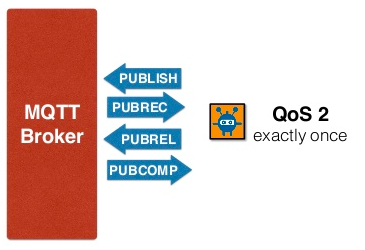
\includegraphics[width=6cm,height=6cm,keepaspectratio]{mqtt_qos2}
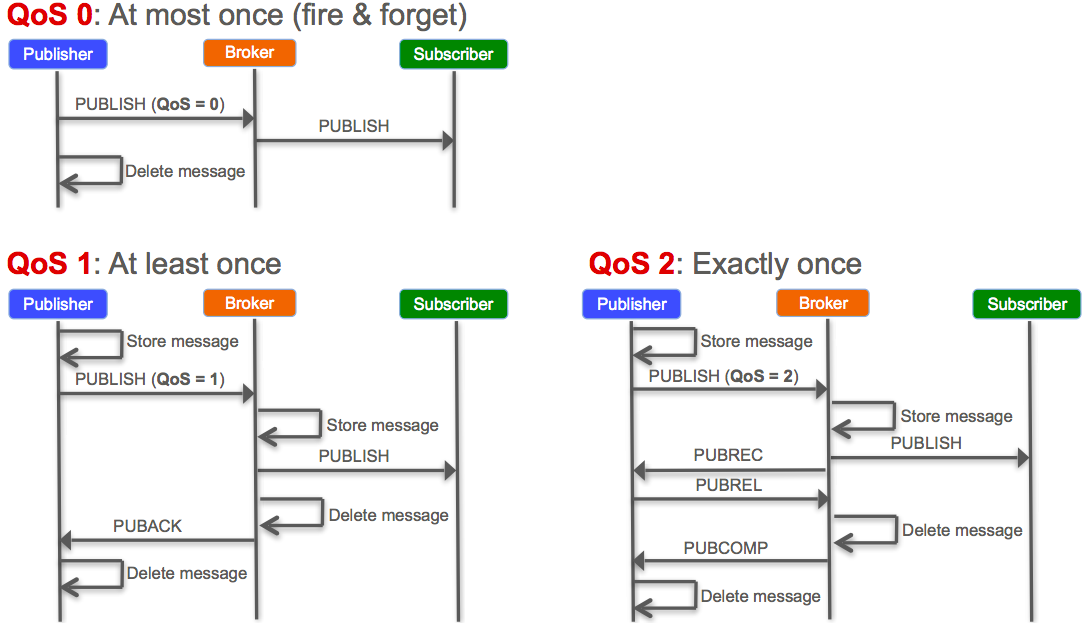
\includegraphics[width=12.5cm,height=12cm,keepaspectratio]{qos_levels}
\centering
\caption{MQTT QoS levels}
\label{fig:qos_levels}
\end{figure}

{\setlength{\parindent}{0cm} {The following real-world examples help to better understand when we should choose one level rather than the others.\\
}

\begin{itemize}
\setlength{\itemindent}{+4mm}
\item if we have a series of solar panels that publish every second some measures on a specific topic, we can accept with no worries that some messages are not delivered correctly, so we may use QoS0.
\item if we have an alarm sensor which publishes an alert message on a topic only if something bad happened in our house, then we want to be sure that such message will be correctly delivered, even more than once, so we may opt for QoS1.
\item if a diabetic person has an auto-injecting insuline device applied to his body, which expects to receive an MQTT message when an extra injection is needed. It is necessary to receive one and only one message, so we must choose QoS2.
\end{itemize}

\bigskip
\subsection{Retained messages}
\bigskip
In MQTT, a retained message is a normal message having the retained flag set to true.
MQTT brokers always store the last retained message received, in order to send it to new subscribers, immediately after subscribing to the corresponding topic.\\\\
What are retained messages useful for?\\

We must remember that MQTT clients are autonomous, therefore they do not know the presence of each other; this means that when a subscriber subscribes to a topic, it has no way of discovering how much time it will take before receiving a message.\\
This problem is solved using retained messages.\\

Example scenario: \\

\emph{if we have a certain device which updates his online status (true/false) on the topic '/devices/devicename/status' only when it changes, and a new subscriber arrives, then he would probably want to be notified immediately about the status of the device.}

\subsection{Persistence}
\label{ssec:mqttpersistence}
\bigskip
MQTT also supports persistence of messages.\\
This feature is very useful because each time a client connects to the broker, a new session for subscribing or publishing to topics is started; if, for any reason, the connection is lost, the process starts all over again with the client establishing a new session.\\
Clearly, this behaviour afflicts the performances of the system, especially when clients have low power and poor connectivity (for instance, intermittent connectivity).\\
A client can request a persistent session setting the \emph{cleanSession} flag within the \texttt{CONNECT} packet to false.\\
Let us notice an important aspect of this feature that we are going to discuss later: to resume a session, the broker has to recognize whether the user is the same as before, and it can do that by using their unique identifier; once the broker finds the match between the clientId and an available persistent session, that session is immediately reassigned to that client.\\

\subsection{Last Will and Testament (LWT)}
\bigskip
It is not uncommon for clients to get disconnected ungracefully from the broker.\\
Therefore, there exist scenarios in which it may be helpful to notify other clients that a specific client has been suddenly disconnected.\\
Thanks to the LWT feature provided by MQTT brokers, clients can choose a message that will be published to previously chosen topics when they get disconnected.\\
As already seen, a client can specify the LWT message as part of the \texttt{CONNECT} packet, then the broker will store the message till it detects that the client has been abruptly disconnected, finally topic's subscribed clients will be notified.\\
Let's clarify that ``ungracefully disconnected" means that a network failure happens, or the client fails to communicate within the keep-alive time, or the client closes the connection without sending a \texttt{DISCONNECT} message or the server faced a protocol error.\\\\
In the real world LWT is often used in combination with retained messages to keep the state of a client updated on a specific topic.\\
For instance, when a client has connected to a broker, it will send a retained message to a topic, named something similar to \emph{``clientname/status"}, with the payload \emph{``online"}.
After that, the client sets the LWT message on the same topic to \emph{``offline"} and, clearly, mark it as retained.\\

\subsection{Wildcards}
\bigskip
A wildcard is simply a shortcut to allow a user to subscribe to multiple topics without having to specify each of them individually.\\

Just to make an example: if the user wants to check the humidity of all his house's rooms, he could simply subscribe to:

$$'sensors/home/+/temperature'$$

to automatically subscribe to topics like the following ones:

$$'sensors/home/livingroom/temperature'$$
$$'sensors/home/kitchen/temperature'$$
$$'sensors/home/bathroom/temperature'$$\\
This first kind of wildcard is called \emph{``single-level"} since it allows the user to avoid to specify one single path level. \\
There is another type of wildcard, called \emph{``multi-level"}, which allows the user to avoid to specify multiple path levels.\\
For instance, both the topics \emph{'sensors/home/livingroom/temperature'} and \emph{'sensors/garage/temperature'} can be subscribed by simply subscribing to \emph{'sensors/\#/temperature'}.\\


\chapter{Security Overview}
\bigskip
MQTT is probably the most used IoT protocol, and experts think it will play an important role in the coming years, therefore it is necessary to talk about its security aspects.\\
Just to begin, we can take a look at its real-world usage in order to understand how much this protocol is widespread, and how many times its security is completely ignored.\\\\
To get this data we use a search engine, called \emph{Shodan}~\cite{shodan}.\\	 
Shodan, developed in 2009, lets the user find specific IoT ``things"(webcams, routers, servers, sensors, printers, traffic lights, etc)  connected to the Internet, providing a huge variety of filters.\\

Thanks to its dangerousness and power, many people call it \emph{``the hackers' search engine"}.\\
Its searching mechanism is based on the so-called \emph{service banners}, which are nothing but metadata sent back to clients by servers: service banners contain a lot of information describing the kind of server/device you are talking to.\\

By default, MQTT brokers listen on port 1883; we can simply find the current visible servers listening on that port by using Shodan and searching for \emph{``port:1883"}.\\\\
On 3rd June 2018 this search produced 160393 results, as shown in figure~\ref{fig:shodanres}.\\

\begin{figure}[H]
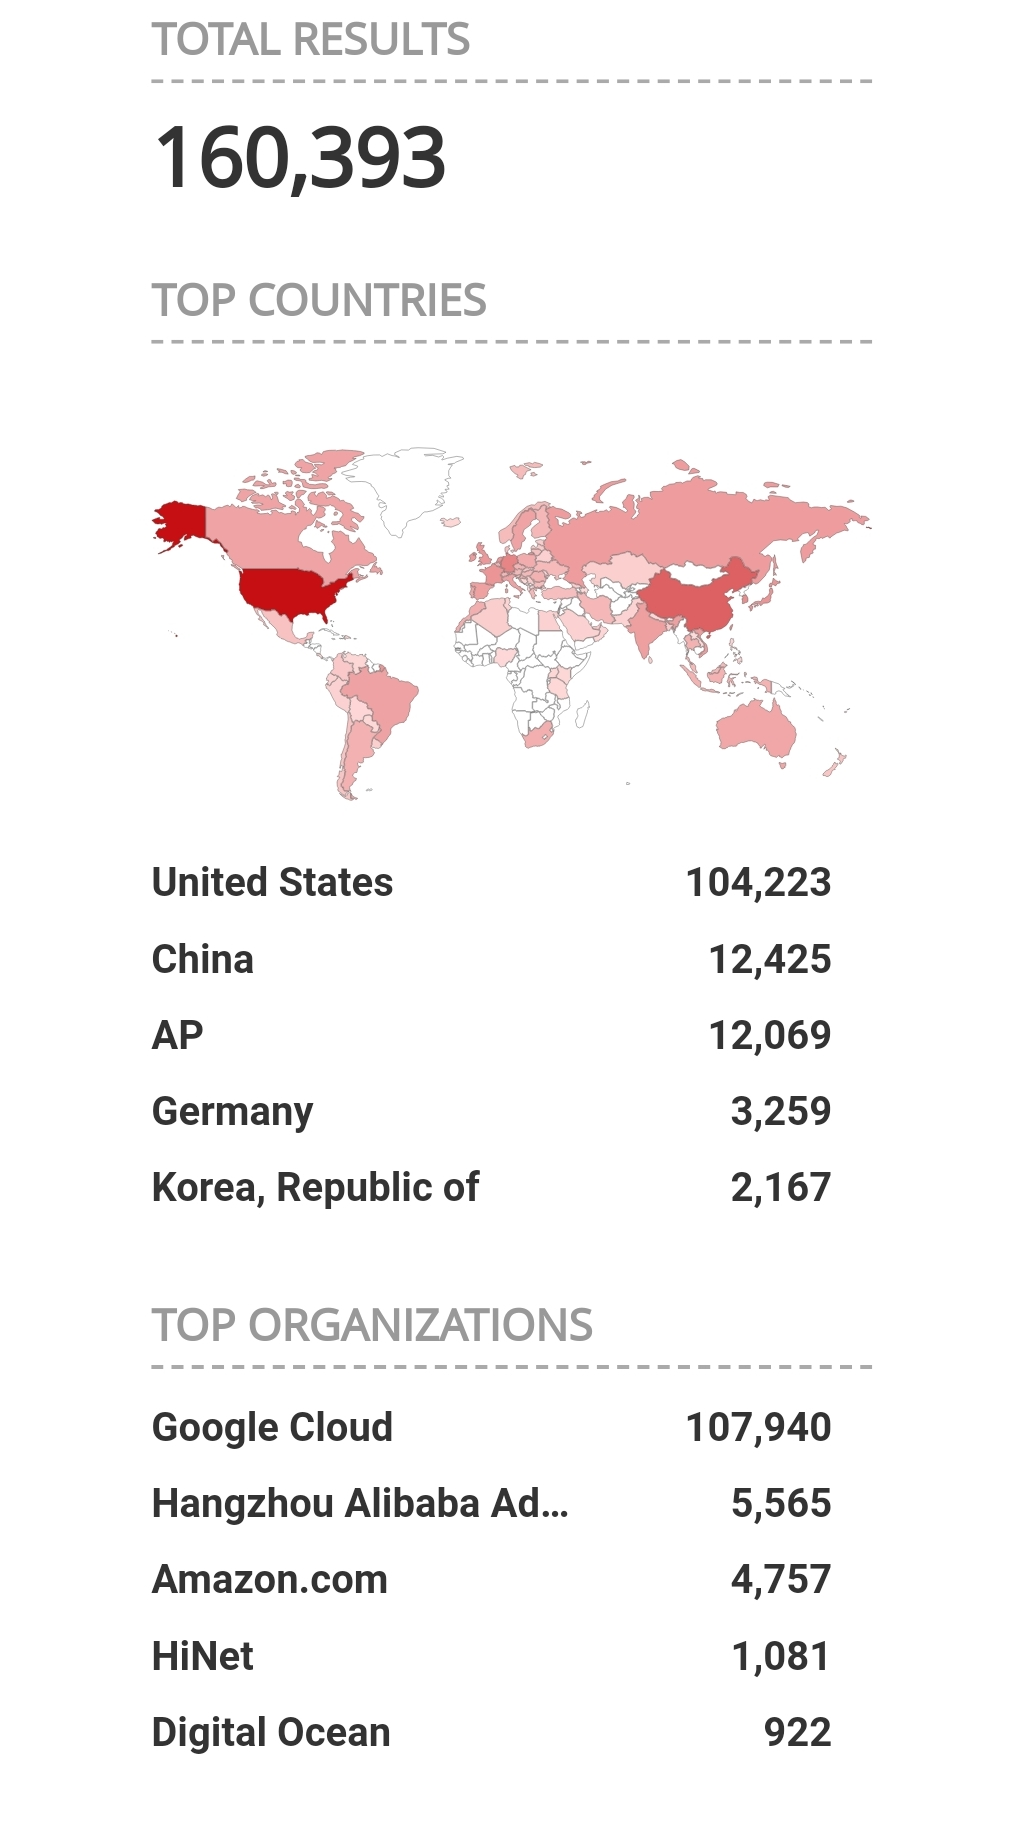
\includegraphics[width=10cm,height=10cm,keepaspectratio]{shodan_numdevices}
\centering
\caption{MQTT brokers found by using Shodan}
\label{fig:shodanres}
\end{figure}\

We found, all over the world, more than 160 thousand devices listening on port 1883, many of them owned by important organizations like Google, Amazon, Microsoft and Alibaba.
While this is already a big number, a more interesting thing is that such a number is growing up very quickly: just two weeks before the same research returned almost 146 thousand devices.\\\\
The port 8883 is standardized for a secured MQTT connection, whose name is ``secure-mqtt", and this port is exclusively reserved for MQTT over TLS.
The first clue that leads us to think that security is neglected is that, if we search again on Shodan, this time filtering on port 8883, we get only 56 servers, so statistically only one broker in a thousand opt for the secure version of the protocol.

Besides, I found a very interesting article on a reliable blog I have been visiting for several years, whose content is strongly related to cyber security\footnote{https://morphuslabs.com/}.\\
An easy-to-implement Python scanner script, exploiting a paid Shodan API key, has been implemented to search for servers listening on port 1883 and then try to connect to them by sending a \texttt{CONNECT} message with no authentication.
The strategy of this attack is pretty simple: the broker we are trying to connect to will reply, as we have already seen, with a \texttt{CONNACK} packet containing the return code; if the return code is equal to 0 it means that the connection has been accepted, therefore the broker leaves the door open to anyone.\\
An analysis conducted on 800 found servers, has led to the following results.

\begin{figure}[H]
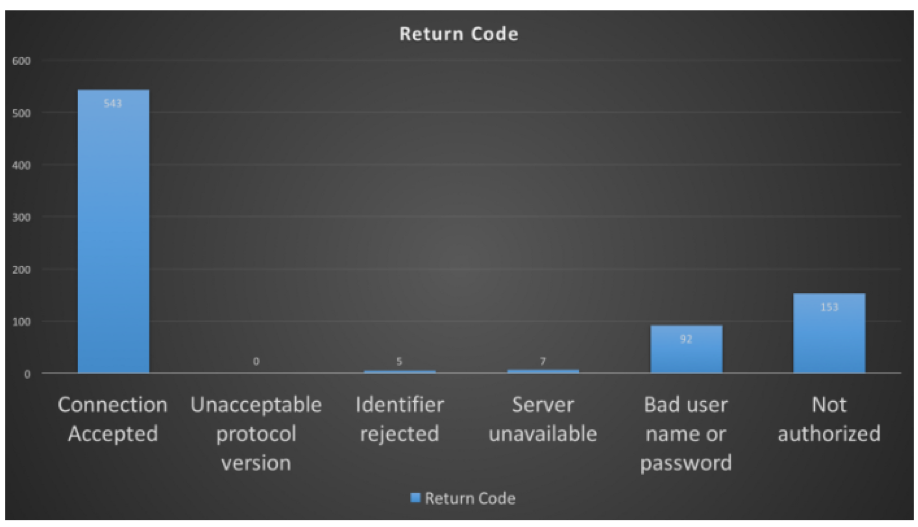
\includegraphics[width=9cm,height=9cm,keepaspectratio]{shodan_results}
\centering
\caption{MQTT brokers return code stastistics}
\end{figure}\
543 brokers out of 800, which is almost 67\%, do not use authentication at all!
\\\\\\\\

\clearpage

\section{MQTT combined with TLS}
\bigskip
Before starting to talk about the authentication methods used by MQTT, we must always remember that MQTT relies on TCP as transport protocol, which means that by default the protocol itself has no built-in encryption.\\
This choice was made purposely by developers to keep it simple, fast and lightweight; therefore, everything is sent in plain text.\\\\
We know that TLS uses an handshake mechanism to negotiate various parameters necessary to establish an encrypted and secure communication which cannot be read or altered by third parties.\\
Usually servers provide their \emph{X.509 certificates}, signed by a trusted authority, to clients to prove their identity.\\
The negotiation of the parameters brings to a communication overhead afflicting performances, requiring more work for the CPUs. This may turn out to be a problem for very constrained devices.\\
Let's suppose to have a constrained device which establishes a new connection every time it has to communicate with the broker; this will bring a huge overhead because the handshaking messages will be the most significant portion of content to send in each communication (considering that usually MQTT devices send simple text messages of few bytes, and the handhsake ones are a few KB).\\
Therefore, it is recommended for constrained devices to use long-living MQTT connections rather than short-living ones in order to drastically improve the TLS performances. This idea is implemented in a technique, called \emph{Session resumption}.

\subsection{Session resumption}
\bigskip
TLS session resumption techniques allow to reuse an already negotiated TLS session after reconnecting to the server; doing this the client does not have to perform the entire TLS handshake again.\\
Unfortunately, some TLS libraries do not implement session resumption, although most of them do.\\\\
There are two session resumption techniques:
\begin{itemize}
\setlength{\itemindent}{+4mm}
  \item[$\bullet$] \texttt{Session Ids}: the server simply stores the secret Session Id associated to a client, so that when this last one reconnects, it provides the Session Id and the session is resumed.
  \item[$\bullet$] \texttt{Session tickets}: the servers send to clients a secret ticket encrypted with a secret key known only by the server.\\
When a client reconnects, it sends its state to the server and if this last one is able to decrypt it, the session is resumed with the state contained in the secret ticket.
\end{itemize}\
Despite everything, very constrained devices do not have enough computational power to support TLS anyway. 
In this case, clients might think to use TLS-PSK cipher suites (not supported by all TLS libraries), since they avoid CPU intensive operations, or totally avoid TLS and use other strategies discussed later.\\\\

To conclude this TLS section, we list some best practices:

\begin{itemize}
\setlength{\itemindent}{+4mm}
  \item[$\bullet$] Clients should always use TLS or, more generically, encrypted communication channels, if they can afford it
  \item[$\bullet$] Use the newest version of TLS, since older ones might have known, and now fixed, bugs~\cite{sslvulns}
  \item[$\bullet$] Always use certificates from trusted Certification Authorities. Using self-signed certificates or allow-all approach is not recommended
 % \item[$\bullet$] Including additional security mechanisms, like payload encryption and authorization mechanisms, in addition to TLS is a good choice.

\end{itemize}

In section~\ref{sec:mqttclientauth} we will talk about client authentication techniques supported by MQTT.

\clearpage
\section{Client Authentication}
\label{sec:mqttclientauth}
\bigskip

There are three ways used by MQTT brokers to verify the identity of a client:

\begin{itemize}
\setlength{\itemindent}{+4mm}
  \item[$\bullet$] Client Id
  \item[$\bullet$] Username and Password
  \item[$\bullet$] X.509 Client certificates
\end{itemize}\

Let's analyze each of them in details.\\


\subsection{Client Id}
\bigskip
We have already seen that clients must include within the \texttt{CONNECT} message a field called \emph{clientId} to identify themselves.\\
This procedure can be, in some way, already considered as a form of authentication since each client must have a unique identifier.\\
It is common practice to use 36-character long identifiers, or some unique information available to the client like his MAC address, or the serial number of the device.
Clearly, this is not secure because someone can easily pretend to be you, just by connecting to the broker specifying your clientId.\\
Depending on the broker's configuration, if the real client has already connected to the broker, the attacker's connection request would be discarded or the real client would be disconnected, but if not, the connection would be certainly accepted.\\

How can the attacker obtain this information? He can easily sniff that, since communication is not encrypted.\\

We have discussed in section~\ref{ssec:mqttpersistence} MQTT persistent sessions, saying that the broker restores the persistent session of a client after he proves its identity specifying its Client Id during connection.\\
This mechanism is not secure by default, in fact an attacker, who have sniffed the unique identifier of the client, can use it to pretend to be him, reads the new messages from his subscribed topics and those sent while it was offline, publishes messages, or simply disable persistence making the real client losing possible important information.\\
Another vulnerability is that the broker stores as much information as possible for clients who have requested persistence, so it stores all the messages from their subscribed topics until it finish its available memory.\\
This behaviour gives an attacker the possibility to connect the broker, requiring a persistent connection, subscribe to as many topics as possible (for instance, subscribing to \emph{'\#'}), then disconnect; doing this, the broker will store a huge number of messages to be sent to the client when it reconnects.\\

Moral of the story: \emph{never rely on clientId to secure your system}.\\

\subsection{Username and Password}
\bigskip
There are two main problems related to this authentication method:

\begin{enumerate}
\setlength{\itemindent}{+4mm}
  \item Since, by default, no encryption system is used, sending credentials is totally pointless, in fact even a trivial \emph{Man In The Middle} attack~\cite{mitmwiki} would be enough to sniff them without effort, as we can see in figure \ref{fig:mqttwireshark}.

\begin{figure}[H]
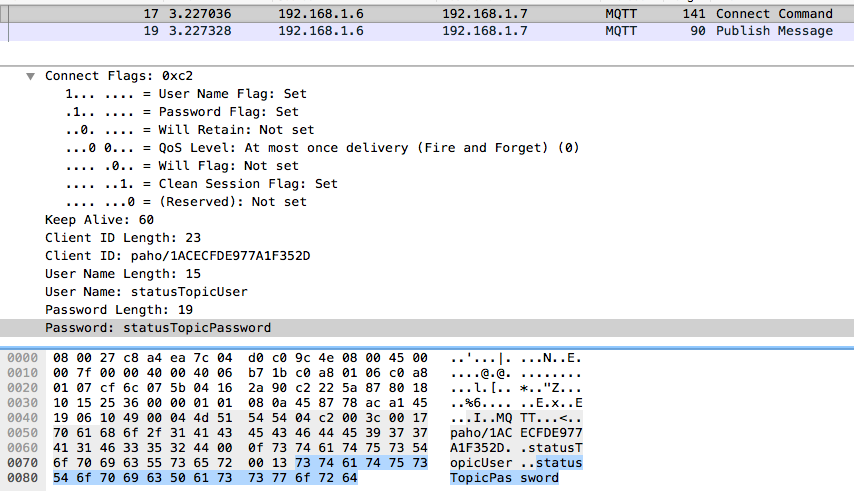
\includegraphics[width=11cm,height=11cm,keepaspectratio]{wireshark_credentials}
\centering
\caption{MQTT credentials sent in plain text}
\label{fig:mqttwireshark}
\end{figure}

\item Authentication is optional, so a huge number of topics are easily accessible from the whole world.\\

The only way to use credentials safely is to combine them with an encrytped communication tunnel (better if TLS).

\end{enumerate}

\subsection{X.509 Client certificates}
\bigskip

Another possible way to identify clients is using their X.509 certificates, which will be sent during the TLS handshake.\\
We are used to servers providing their X.509 certificates to clients to prove their identity, and clients authenticating in the application layer.\\
In this case, however, we perform \emph{mutual authentication}, since client and server authenticate each other at the same time using X.509 certificates.\\
The broker will use the information in the certificate for application layer authentication after the TLS handshake has completed with success.\\

This authentication method is very secure but rarely used because it requires the provisioning and managing of the certificates to the clients, besides this double negotiation afflicts even more the performances.\\

Now, let's take a look at pros and cons of using client certificates.
\begin{itemize}
\setlength{\itemindent}{+4mm}
\item[$\bullet$] Pros:
\begin{itemize}
\item only valid clients are allowed to establish a secure connection
\item authentication of clients at transport level, so invalid clients are discarded before \texttt{CONNECT} messages are sent.\\ 
This is very useful to save resources on broker's side, because authentication mechanism can be expensive (a common case is that credentials are stored in a database, which must be interrogated every time someone wants to connect) and using client certificates makes them useless.
\end{itemize}

\item[$\bullet$] Cons:
\begin{itemize}
\item Managing a huge number of client certificates may be a serious burden, therefore it is important to have a solid certificate provisioning process. In other words, clients' certificates must be kept updated, and owners should have a way to manage their lifecycle.
It is suggested to use certificates, only when clients are under their strict control.
\item It could happen that a client's certificate get leaked and, consequently, cannot be trusted anymore since some attacker may use it, so it is necessary to have a way to revoke invalid certificates.\\
There are two ways to obtain that:

\begin{enumerate}
\item \emph{Certificate Revocation Lists (CRLs)}: they are simple lists of certificates that have been revoked before their expiration.
These lists are created and continuously updated by the related Certification Authority.
A server hosting a broker can have its own local CRL to consult, but clearly it has to get updates from the CA, from time to time.\\
This is not a very convenient procedure.
\item \emph{Online Certificate Status Protocol (OCSP)}:  it is a protocol used for asking information about specific client certificates, more specifically to know if they are still trustable.\\
In order to use OCSP there must be a so-called \emph{OCSP Responder}, which is an HTTP server waiting for revocation-check requests, provided by the certification authority.
This is a better and faster solution since you do not have to download the entire, and possibly huge, list every time before checking a certificate.\\
Let's see a simple example~\cite{ocspwiki} of how it works:

\begin{itemize}
\item Alice and Bob want to communicate and have their certificates issued by a certification authority, called Carol
\item Alice starts the transaction by sending her certificate to Bob 
\item Bob, who suspects that Alice's private key might have been compromised, sends an \emph{OCSP request}, containing Alice's certificate serial number, to Carol
\item Carol's OCSP responder search in its database the certificate's serial number received from Bob
\item At this point, Carol's OCSP responder returns a signed successful \emph{OCSP response} to Bob if the certificate is still valid, otherwise will reply telling Bob that the certificate is not valid anymore
\item Depending on the response received by Carol, Bob will decide whether carry on, or not, the communication with Alice.\\
\end{itemize}


\end{enumerate}
\end{itemize}
\end{itemize}


To sum up, this kind of authentication is secure but expensive, therefore only suited to a small number of clients which need high security. \\

In section~\ref{sec:mqttauth} we will discuss authorization, another important concept related to security.\\


\section{Authorization}
\label{sec:mqttauth}
\bigskip
Authorization and authentication go hand in hand, but they are very different security concepts.\\
While authentication is used to recognize the identity of a client, authorization allow us to create policies in order to restrict access to certain resources (\emph{in this scenario resource means topic}).\\

In MQTT, without authorization, every authenticated client could do whatever he wants, so publish or subscribe to any existent topic.\\
More in details, the resources to protect are the common actions: publishing, subscribing, setting a LWT or retained message, requiring a persistent session.\\\\
How can the broker restrict permissions on topics?\\

Brokers can limit clients' permissions implementing some authorization policies called \emph{topic permissions}, having, at least, the following information:

\begin{itemize}
\setlength{\itemindent}{+4mm}
  \item[$\bullet$] Allowed topic
  \item[$\bullet$] Allowed operations (publish, subscribe, LWT, retained messages)
  \item[$\bullet$] Allowed quality of service levels (0, 1, 2, all)
\end{itemize}

What does it happens when a client tries to access a restricted resource without having enough permissions?\\

If the client tries to publish, the broker can disconnect it or simply reply to it normally, but without relaying the message to subscribers; instead, if the client tries to subscribe, the broker will reply with a standard \texttt{SUBACK} message containing a return code that tells the client that its subscription was denied, nothing more.\\

In section \ref{sec:mqttauth2} we discuss another form of authentication/authorization mechanism usually implemented in other protocols, like HTTP, and we will see wether and how it is possible to combine it with MQTT. 


\section{Simple Data Encryption}
\bigskip

In this section we discuss a workaround to grant secrecy of messages without involving TLS: encrypting ony sensitive data, such as the payload in \texttt{PUBLISH} messages.\\

Using this strategy sensitive data, let us assume the payload in our examples, will be encrypted, but other metadata remains unencrypted.\\
Notice that the broker has no decryption key, so it will relay the messages to subscribers as is, without knowing their real content.\\
Clearly, this mechanism expects subscribers to have the proper key to decrypt the received payload.\\

Figure \ref{fig:endtoend} explains this scenario, called \emph{End-to-End}, perfectly.

\begin{figure}[H]
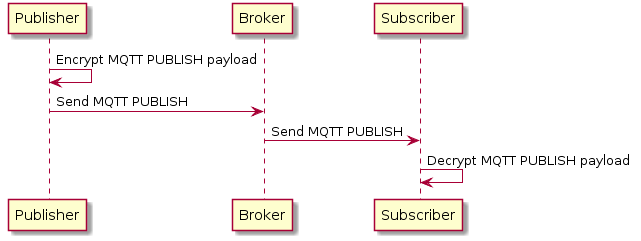
\includegraphics[width=12.5cm,height=12cm,keepaspectratio]{end_to_end}
\centering
\caption{MQTT communication using End-to-End encryption}
\label{fig:endtoend}
\end{figure}

Now, a question arises: if we encrypted meta data, like client's credentials in the \texttt{CONNECT} packet, how could the broker decrypt and validate them?
This is a very uncommon practice, because it requires to write an additional plugin for the broker in order to make it able to decrypt our data. 
This second scenario is called \emph{Client-to-Broker}.\\
In this case, the broker will send the decrypted message to subscribers, which will not have to know any key, as we can see in the following figure \ref{fig:mqttclienttobroker}.

\begin{figure}[H]
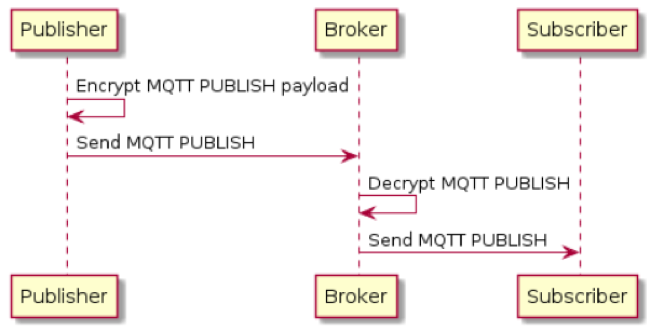
\includegraphics[width=10cm,height=10cm,keepaspectratio]{client_to_broker}
\centering
\caption{MQTT communication using Client-to-Broker encryption}
\label{fig:mqttclienttobroker}
\end{figure}

Should we use an asymmetric or symmetric encryption scheme to encrypt the payload in a \texttt{PUBLISH} message? We should

\begin{itemize}
\setlength{\itemindent}{+4mm}
\item[$\bullet$] prefer asymmetric cryptography when we have many, possibly untrusted, publishers and few trusted subscribers, because these last ones know the private key which is used to read the messages in the subscribed topics.
In this way, only trusted clients can decrypt the topic's messages.
\item[$\bullet$] use symmetric cryptography when we have a trusted environment, in fact we must remember that in this case there is only one key to encrypt and decrypt, so we can share it with everyone.
\end{itemize}
\bigskip
Certainly, using a single symmetric key is simpler to implement, but less flexible.\\

We conclude this section wrapping up the pros and cons of data encryption:

\begin{itemize}
\setlength{\itemindent}{+4mm}
\item encrypting only specific data is a method to add a security layer to communication, and can be an option for constrained devices which cannot rely on TLS.
\item[$\bullet$] encrypting and decrypting every message can be intensive for constrained devices, in fact it is fundamental to choose a fast encryption algorithm
\item[$\bullet$] we must remember that encrypting only specific data prevents attackers to sniff our sensitive information, but man in the middle attacks, as well as replay attacks, are still possible.\\ 
Just to make an example: an attacker could intercept a valid message and modify some parts of it, like the topic
\item[$\bullet$] keys management adds a layer of complexity, for instance it is important to establish a secure provision of them.
\end{itemize}
\bigskip

\clearpage
\section{Data Integrity}
\label{sec:dataintegrity}
\bigskip

We previously described tokens and how their signatures are used to make sure they have been generated by a trusted source, like the Authorization server; now, we see, in general, how brokers can validate received messages.\\
Data integrity is fundamental because it is the only way to assert that the content of a message is authentic and has not been altered by third parties.\\
There are three different approaches for message integrity checks:

\begin{itemize}
\setlength{\itemindent}{+4mm}
\item[$\bullet$] \emph{Checksum}: a value calculated, with a series of calculations that converts the message payload into a string of digits.\\
This value is sent with the payload, so the receiveing application has just to recalculate the checksum to verify the integrity of the message.\\
This approach guarantees that data was not modified by a transmission error, but it cannot assure that it comes from a trusted sender.

\item[$\bullet$] \emph{Message Authentication Code (MAC)}: this authentication code is calculated using a \emph{HMAC} combined with a cryptographic key. Since only trusted clients know the secret key, we can discover if a message come from a trusted client or not. \\
\emph{HMAC} is very fast compared to digital signatures.\\
Clearly, this second authentication way involves a key, so there must be a provisioning way.

\item[$\bullet$] \emph{Digital signature}: it is a code generated by a public key encryption algorithm. More in details, the client signs the message with its private key and the broker validates the signature using the public key of the client.\\
This approach is the most secure because the only way to sign a message properly is knowing the private key, which is known by the real client only, but at the same time the broker has not to know it too.\\
So, this approach guarantees the same things of the previous one plus the certainity that a specific user sent the message.\\
The difference with respect to the previous approach is that the secret key was shared to all clients, while in this case each client has its own private key, but the broker is still able to decrypt their messages using their public key.\\
\end{itemize}

Secrecy combined with integrity gives the system a robust security: secrecy prevents attackers to see our things, and integrity prevents attackers to alter them without being discovered.\\\\

%In section \ref{sec:mqttsdp}, we see how to make a MQTT system even more secure by using a not very common, but very powerful, security architecture called \emph{Software Defined Perimeter}, or simply \emph{SDP}.\\


\section{MQTT combined with an SDP}
\label{sec:mqttsdp}
\bigskip
In this section we describe a sophisticated solution to implement a very secure MQTT system; since this architecture's implementation seems to be a bit difficult, it should be taken into consideration only if your system needs to be very protected.\\

\subsection{What is an SDP?}
\bigskip
An \emph{SDP (Software Defined Perimeter)}, also known as \emph{Black Cloud}, is an emerging security architecture, a bit difficult to implement and manage, that restricts accesses and connections among allowed devices.\\
Once, companies used to define a local physical network perimeter in order to protect their applications from external threats.\\
Nowadays, digital progress has significantly broadened these boundaries, and IoT is the biggest proof of that, in fact having sensors scattered in different places of the world make it impossible to define a local physical network as it used to be.\\

SDP relies on a strategy based on \emph{``hidden-resources"}, or \emph{``non-visibility"}, to provide secure access to devices and applications.\\
A traditional internal network separated by the external world has a well-defined perimeter and makes use of some firewall functions denying the access to external users, but allowing internal ones to communicate with the external world.\\
Instead, an SDP is a scalable solution able to provide a secure and authorized access to resources in a perimeter in continuous evolution.\\

\emph{We may think to a network protected by an SDP like a private and exclusive society distributed all over the world, where everybody would like to access, but to which only authorized persons will access.}~\cite{protectnetwithsdp}\\\\
It is important to say that SDPs are not strictly connected to IoT technologies, but they can be used in different fields.\\

\subsection{How does an SDP work?}
\bigskip

Devices trying to access are first identified, then, once they have been accepted within the protected network, they are subjected to a further verification process, an authentication with credentials, and finally are assigned permissions based on their authorizations.\\
Let's see more in details how it works.\\

First of all, an SDP expects a secure connection, therefore encrypted, based on a \emph{``need-to-know"} logic, that allows only identified, authenticated and authorized clients to access network resources.\\
There exist many different SDP structures, as we will detail in the following, but they all refer to the idea of \emph{``hide to protect"}.\\\\

Figure \ref{fig:sdpstructure} shows an example of a possible SDP structure.

\begin{figure}[H]
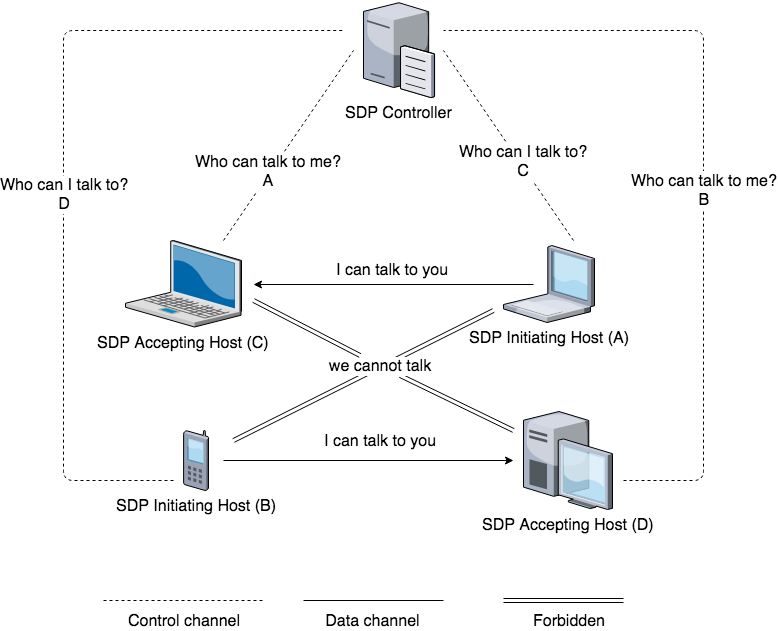
\includegraphics[width=10cm,height=10cm,keepaspectratio]{sdp_structure1}
\centering
\caption{Example of  SDP structure}
\label{fig:sdpstructure}
\end{figure}

There are two components: \emph{SDP Hosts} and \emph{SDP Controllers}; SDP Hosts can either initiate or accept connections, and these actions are managed by interactions with the SDP controllers through a secure control channel.\\
This is a possible SDP workflow:

\begin{enumerate}
\item One or more Controllers are brought online and connected to the appropriate authentication/authorization services
\item Hosts, after being brought online, connect and authenticate to the controllers and, for the moment, they do not accept to communicate with any other host
\item Controllers determine a list of Accepting Hosts to which the Initiating Hosts are authorized to communicate
\item Controllers instruct the Accepting Hosts to accept connection from the Initiating Hosts and gives these last ones the list of Accepting Hosts.\\
Since we said that communication is encrypted, policies containing infomation about encryption are sent to both Accepting and Initiating hosts.
\item Now Initiating Hosts can communicate with Accepting Hosts.\\
\end{enumerate}

\subsection{How can this architecture be combined with MQTT?}
\bigskip
%Before describing how we can make SDP working with MQTT, let's clarify that the SDPs we are going to see are not exactly like the one in Figure \ref{fig:sdpstructure}; they are similar, since they follow the idea of ``hide to protect", but simpler.\\

We have seen that MQTT allows clients to specify username and password while connecting to a broker.\\By using an SDP, the pair username/password could be replaced using the so-called \emph{Single Packet Authorization (SPA)}~\cite{mqttonlywithsdp}.\\

What is a Single Packet Authorization?~\cite{portknockandspaanalysis}\\

SPA is a technique to securely get access to certain service ports, communicating across closed firewall ports.\\
So, the initial idea is to make services unaccessible to the outside keeping all the server's ports closed, or at least those ones where services to protect are listening on.\\

SPA is a kind of evolution of an older system called \emph{Port Knocking}, in which we are able to  open some closed firewall ports from the outside by sending connection attempts to a pre-established sequence of closed ports; then the firewall updates its own rules in order to allow the sending host to connet to the desired port.\\
This old system is basically flawed and vulnerable to replay attacks, as we can see in Figure \ref{fig:portknocking}, in fact an attacker can sniff the attempts and replay them, obtaining the access to the service's port.\\

\begin{figure}[H]
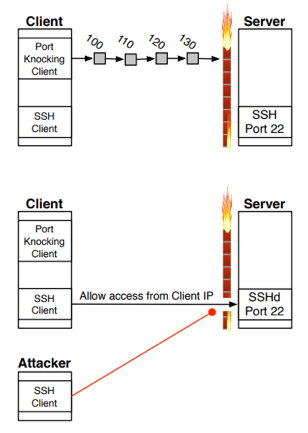
\includegraphics[width=9cm,height=9cm,keepaspectratio]{port_knocking}
\centering
\caption{Port Knocking Replay attack}
\label{fig:portknocking}
\end{figure}

SPA and Port Knocking have the same goal but quite different delivery mechanisms: in this newer system, as the name suggests, all of the necessary information, the so-called ``knock", is encoded in a single \emph{Authorization Packet}.\\
This AP can be sent using TCP, UDP or ICMP, but usually these last ones are preferred.\\
An AP has the following simplified structure:

\begin{itemize}
\setlength{\itemindent}{+4mm}
\item[$\bullet$] \texttt{Timestamp}:1523357581
\item[$\bullet$] \texttt{Client IP}: 2.225.190.3
\item[$\bullet$] \texttt{Password}: somethingsecure
\end{itemize}

Then, what is actually sent to the server is a resulting MD5 hash calculated in this way:
\small
$$ \texttt{MD5(\$timestamp:\$client IP:\$password) = 35b45e73c99905b675ffb05b78714eb9} $$

\normalsize
Once the server received the packet, a SPA daemon will recalculate the hash starting from the password, which must be known from both the client and server, the IP address of the client and the current timestamp.\\
If the resulting hash matches the received one, then the firewall allows that specific client IP to connect to the desired port, otherwise no action is performed.\\
So, we have some advantages using SPA:

\begin{itemize}
\setlength{\itemindent}{+4mm}
\item[$\bullet$] we do not have to respect a certain packet delivery order.\\
It does not seem to be such a big problem, but it is not so unlikely to make it wrong since the server does not send any acknowledge packet back while receiving knock
\item[$\bullet$] the timestamp and client IP within the AP prevent replay attacks
\item[$\bullet$] the use of the password increases security, but clearly there must exists a way to share it with authorized clients
\item[$\bullet$] encoding the packet using MD5 makes almost impossible for attackers to steal the secret password, when the password is properly chosen
\end{itemize}

All these precautions make attackers' life very hard.\\

Coming back to MQTT, we said that username and password could be replaced with an SPA.\\
Applying what we have just discussed to MQTT security, we may think to hide devices, so that they cannot be seen by attackers, and let them communicate just with pre-established brokers.\\
On the other side, we will let brokers communicate only with clients who send a valid Authorization Packet.\\\\
To make it a bit more secure, we may think to give the broker a list of authorized IP addresses, and reject the communication with any IP not contained in this list, even if able to send a proper AP.\\
Clearly, the bad aspect of this restriction is that it is less scalable and IP addresses can be spoofed.\\

Once a (valid) client have sent a proper AP, the server hosting the broker will allow it to connect to the MQTT dedicated port, and finally the broker will receive messages from it.\\
The MQTT port will remain open for a certain (little) period of time, after which the client will have to send another AP to get authorization.\\

We notice that this system is robust even without TLS, and this might be the proper choice to authenticate devices unable to support it, but the problem persists after the authentication: it is true that only messages coming from trusted clients are received by the broker, but the messages following the authentication are still vulnerable to MITM attacks.\\

As always, using TLS is the best solution, but if not emplyable we may face this problem with a workaround, but keeping in mind that \emph{it should be considered only if TLS is absolutely impossible to use}: since authorized users already know the secret password, using it as input for a key derivation function to obtain a cipher key might be an idea.\\


\section{Best practices}
\label{sec:mqttbestpractices}
\bigskip
Combining all the things we have discussed so far, we can try to list some best practices to consult before creating a secure MQTT system.
\bigskip
\begin{itemize}
\setlength{\itemindent}{+4mm}
\item[$\bullet$] Protect communication using encryption; use TLS whenever possible, otherwise encrypt sensitive data and grant data integrity using one of the techniques we have previously described.\\
If we use TLS, we must remember that commonly used TLS is already secure enough, but it only proves the identity of the server to the client using a X.509 certificate, while the authentication of the client to the server is left to the application layer.\\
If we want to strengthen even more this mechanism, we may think to use mutual authentication, so, as already discussed, the client will send its own X.509 certificate to the server to prove its identity.\\
This choice can afflict performances.
\item[$\bullet$] Request clients authentication.%, that is using credentials to login to a broker. This step is optional, since the client has already authenticated on the server sending the AP, and it seems to be a bit redundant but it might be an additional option.
\item[$\bullet$] Disallow client authentication through clients identifiers.
\item[$\bullet$] Disallow access to system topics. They can contain information about the connected clients, including their identifiers.
\item[$\bullet$] Define properly the authorizations to assign to clients, such that once a server accepted a client connection, this last one must have access only to authorized resources, that are brokers, specific topics and, even deeper, actions allowed on these ones (publish, subscribe, LWT, retained messages).
\item[$\bullet$] Use \emph{Throttling}, that means limiting the total incoming bytes per second on a global or a per-client basis, in order to spare bandwidth.
\item[$\bullet$] Think about a good load balancing: a large MQTT system may distribute the traffic to multiple MQTT brokers rather than just one, to avoid work overloads.\\
There are many tools to automatize this mechanism, called load balancers and most of them are also able to detect unusually high traffic and block it.
\item[$\bullet$] Define the maximum message size (the default one is 256 MB)
\item[$\bullet$] Choose the proper QoS level according to your needs.
\item[$\bullet$] Check you server and its operating system.
\item[$\bullet$] Keep software and libraries updated.\\
\end{itemize}

If you also plan to combine MQTT with an SDP, you should:

\begin{itemize}
\setlength{\itemindent}{+4mm}
\item[$\bullet$] Hide devices and limit access to resources/services using SPA with a secure enough password (in this case, secure enough means not vulnerable to brute force and dictionary attacks: attackers must not be able to get accepted from the server trying a huge number of generated passwords or taken by a list)
\item[$\bullet$] Define properly who can communicate with whom: specifically, servers hosting brokers must accept only connections from clients able to send a proper AP. As already said, if our goal is to have a very strong system, the server can keep a list of accepted client IPs, and immediately truncate connections from unregistered ones, even if valid APs are sent; the same is true for clients, so each client must have a list of servers with which is allowed to communicate.
\item[$\bullet$] Define an authentication password to specify within the APs, and how to share it with registered clients at the beginning
\item[$\bullet$] Use tools to detect brute force/dictionary attacks and lock out attackers.
\end{itemize}

%In the next section, we will try to apply in practice the theoritical concepts seen so far, developing an homemade secure MQTT system.\\

\section{Homemade secure MQTT system}
\label{sec:homemademqtt}
\bigskip
This example can be seen as a kind of pratical guide of how to build a \emph{simplified} homemade secure MQTT system.\\
Before starting, let's see a list of the technologies we are going to use:
\bigskip
\begin{itemize}
\setlength{\itemindent}{+4mm}
\item[$\bullet$] OS: Ubuntu 16.04 Desktop
\item[$\bullet$] Programming languages: Python, NodeJS, Bash
\item[$\bullet$] Redis, Iptables, openssl, Nmap\\
\end{itemize}

By using this minimal set of technologies, we can build a quite secure MQTT system. In details, our goals are:\bigskip
\begin{itemize}
\setlength{\itemindent}{+4mm}
\item[$\bullet$] creating a simple MQTT broker
\item[$\bullet$] making server's resources/services hidden to everyone and accessible only by registered, authenticated and authorized client IPs, by using the SPA strategy we have discussed before
\item[$\bullet$] implementing a bruteforce/dictionary attack detector, able to block attackers
\item[$\bullet$] making clients talk only with the server
\item[$\bullet$] encrypting MQTT messages with TLS
\item[$\bullet$] looking at an example of publish/subscribe specifying the desired QoS level and retained messages\\
\end{itemize}

Clearly, \emph{this is just a simplified demo}, therefore we will make some assumptions along the way.\\

Let's start understanding how to hide resources.

\subsection{Hiding resources}
\bigskip
The first step for the server to avoid connections from/to undesired client IPs is to properly configure its firewall, adding the correct constraint rules.\\
Assuming our tiny system is composed by the following actors:
\bigskip
\begin{itemize}
\setlength{\itemindent}{+4mm}
\item[$\bullet$] Server (\emph{192.168.1.126})
\item[$\bullet$] Client 1 (\emph{192.168.1.6})
\item[$\bullet$] Client 2 (\emph{192.168.1.7})\\
\end{itemize}

Let's start creating a simple text file containing the list of registered client IPs; let's call it ``\texttt{trusted\_client\_ips.txt}".\\
Then, we move on blocking all the incoming and outgoing connections, except for the ones from/to the registered client IPs on the SPA dedicated port.\\\\
To do that, we simply write two bash scripts to properly configure the server and clients' firewall using nothing more than iptables.

\clearpage
\begin{center}
  \lstset{%
    caption=Server's firewall configuration script,
    basicstyle=\ttfamily\small\bfseries,
    frame=tb
  }
  
\begin{lstlisting}[language=bash]
#!/bin/sh
iptables -F
iptables -P INPUT DROP
iptables -P OUTPUT DROP
file="trusted_client_ips.lst"

while IFS= read line
do
   iptables -A INPUT -s $line -p tcp --dport 62015 -j ACCEPT
   iptables -t filter -A OUTPUT -d $line -p tcp -j ACCEPT

done < "$file"

iptables -nL
\end{lstlisting}
\end{center}

The code above shows the bash script used to configure the server's firewall; the client's script is almost identical, but \emph{OUTPUT} becomes \emph{INPUT} and viceversa, finally the filename changes to \emph{``trusted\_servers.lst"}.\\


The dedicated port is the only open port on the server, running the Python daemon responsible to accept only registered IPs messages and verify if they are valid APs.\\
%\underline{Note}:  an attacker might try to perform brute force or dictionary attacks against this daemon, so we will explain later how to easily protect our system from them.\\

\subsection{SPA mechanism implementation}
\bigskip

The SPA daemon is a simple Python server which accepts only connections from authorized client IPs and discard all the others.\\

Once the daemon receives an AP, it simply uses the pre-established password, the IP address of the sender and the current timestamp to generate the expected MD5, then it compares it with the received one, and if they are equal the received AP has to be considered valid.\\
All of this stuff can be done in few lines of code:\\

\begin{python}

service_port=8883
log_filename="SPA_daemon.log"
SPA_passwd="supersecretpassword"

def grantAccessToClient(client_ip):
  cmd1="iptables -I INPUT -s %s -p tcp --dport %s -j ACCEPT" %(client_ip,service_port)
  
  cmd2='echo "iptables -D INPUT -s %s -p tcp --dport %s 
        -j ACCEPT"|at now+2 minute;' %(client_ip,service_port)
        
  os.system(cmd1)
  os.system(cmd2)                                      
                                         
                                                            
def checkAP(received_md5,client_ip):
  timestamp = str(time.time())
  timestamp = timestamp[0:timestamp.find('.')] # avoid ms
  str_to_encode="%s:%s:%s" %(timestamp,client_ip,SPA_passwd)
  expected_md5=hashlib.md5(str_to_encode).hexdigest()

  if(expected_md5==received_md5):
    grantAccessToClient(client_ip)
  else:
    log_file.write("[%s] %s - Invalid MD5 received\n"        %(timestamp,client_ip))
    log_file.seek(0)
  
\end{python}
\bigskip

The idea is pretty simple: if the daemon receives a valid AP, it adds an Iptables rule to allow the client to access the service port, otherwise it does nothing.\\
\underline{Note}: since we want the access to the service to be limited in time, we run the command \emph{``at"} which gives us the opportunity to run a command after a certain period of time (in the example it is 2 minutes, but in a real scenario it should be larger). Another thing we should notice is that we log only the negative cases, and we do this because there is another script which makes use of this log file to detect and block bruteforce/dictionary attacks in real-time.\\

This detector implements a very simple but effective detection strategy: when it reads a new line of the daemon's log file, it takes the client IP address and checks if the number of invalid APs received by it in the last \textsc{time\_range} minutes is larger than \textsc{max\_requests}; if so, that client IP is locked out for \textsc{ban\_time} hours, and to do that it simply adds an iptables rule again.\\
This last rule will expire automatically using once again the command ``at" to delete it from Iptables.\\
Of course, it is important to define properly these constants: let's say, for instance, that we may accept at most 5 invalid APs for IP in the last 30 minutes and ban the user for 6 hours.\\

We skip the analysis of the SPA client because it is nothing but a Python script sending well-formed requests to the server's daemon through sockets.\\

Instead, we can see in Figure \ref{fig:nmapproof} a proof of how this SPA mechanism works well, using Nmap to scan the service port, which is the 8883, on the server before and after sending a valid AP.

\begin{figure}[H]
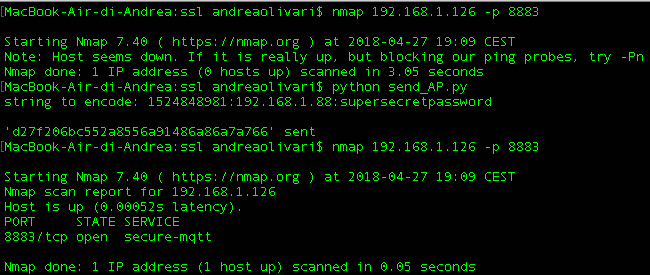
\includegraphics[width=13cm,height=12cm,keepaspectratio]{nmap_proof}
\centering
\caption{Nmap scan before and after sending a valid AP}
\label{fig:nmapproof}
\end{figure}

Of course, we have to run a broker on the port 8883, and I have done that using an easy-to-use nodeJS module, called \emph{Mosca}~\footnote{https://github.com/mcollina/mosca}.\\ 

Mosca gives the user the opportunity to use TLS as well as credentials and two storing methods: MongoDB or Redis.\\
I opted for \emph{Redis} (\emph{REmote Dictionary Server}), which is  nothing but a key-value store with optional durability, often used to cache server content that needs to be accessed quickly.\\
We skip a deep analysis of the broker's code since it is very similar to the example you can find in the module's page, except for some security constraints we added:

\begin{center}
  \lstset{%
    caption=Mosca broker security settings,
    basicstyle=\ttfamily\small\bfseries,
    frame=tb
  }
\begin{lstlisting}[language=javascript,caption=Mosca broker security settings]
var moscaSettings = {
  port: 8883,
  backend: listener,
  persistence: {
    factory: mosca.persistence.Redis
  },
  secure: {
    keyPath: "broker_cert.key",
    certPath:"broker_cert.pem"
  }
};

var server = new mosca.Server(moscaSettings);

server.on('ready',function() {
  console.log("MQTT broker is up and running");
  server.authenticate = function(client,username,password,callback) {
    callback(null,(username===broker_username && password.toString('ascii')===broker_password))
  }
});
\end{lstlisting}
\end{center}

We have added the authentication control and enabled TLS specifying two files, \emph{broker\_cert.key} and \emph{broker\_cert.pem}, where the first one contains the broker's certificate private key, while the second is the server certificate to be sent to the client, containing the public key of the server.\\
Clearly, in order to use this certificate, we first have to create it: it is possible to create self-signed X.509 certificates using the Linux command \emph{``openssl"}.\\

In this demo our MQTT broker uses a self-signed certificate generated locally and I properly configured clients to consider it as trustable, but \emph{in a real scenario we have to rely only on trusted certification authorities, so this is absolutely forbidden}.\\

At this point, MQTT clients can be implemented using Python once again, and more in details its library \emph{paho.mqtt} (available also in Java and other programming languages), to simply connect to the broker and publish/subscribe to topics.\\
This library is easy to use, and allows us to set TLS, credentials, QoS levels and retained messages in no more than one line of code for each feature:\\

\begin{python}
def publishMsg(client,topic,message,qos_level,retain_msg):
  client.publish(topic,payload=message,qos=qos_level,        retain=retain_msg)

client = mqtt.Client()
ssl_version = ssl.PROTOCOL_TLSv1_2
client.username_pw_set(brk_username,password=brk_password)

client.tls_set("broker_cert.pem",cert_reqs=ssl.CERT_REQUIRED,  tls_version=ssl_version)
publishMsg(client,topic_pub,"online",1,True)
\end{python}


\chapter{Real-world examples}
\bigskip
I did my internship working for four months with a company called ABO DATA, which deals with IoT technologies.\\
The company enables customers to customize and manage IoT business applications: most of the times we talk about customers' devices/sensors which send their measurements to a cloud or a centralized system, then these measures are computed and exploited to do something else related to customers' business.\\
So, during my internship I often had to deal with tasks related to receiving data from a source and their subsequent forwarding to a destination, like a bridge, typically using two protocols: HTTP(s) and MQTT.\\

In Section \ref{sec:intership_case1}, I would like to discuss two real-world cases I have worked on, which should make us reasoning about how a production system should be thought and implemented.\\

\clearpage
\section{Case 1 - Real-world MQTT-based industrial system}
\label{sec:intership_case1}
\bigskip
This is a real-world scenario involving an important company, whose name cannot be disclosed for reasons of privacy, partner of several automotive, pharmaceutical, writing tools and watchmaking industries, that produces and distributes automated systems as well as high-precision and efficient cutting tools.\\

This company recently decided to build a realiable monitoring and management system for their machines using a \emph{cloud} architecture.\\
The requirements were to collect data from machines' sensors in order to create a so-called:

\begin{itemize}
\setlength{\itemindent}{+4mm}
\item[$\bullet$] \emph{Local Control Room}, which allows the company's customers to check the performances, real use and health status of their machines, in real-time
\item[$\bullet$] \emph{Centralized Control Room}, which allows the company itself to monitor their resources operating with different customers in order to collect historical data, useful to make analysis and comparisons
\end{itemize}

These monitoring systems collecting tons of data are often used by companies and industries to drastically change and improve their maintenance approach.

A \emph{Time-based} maintenance approach is the simplest one, and unfortunately the most used, so when a machine breaks down, the customer contacts the support company to receive assistance.\\
The use of a monitoring system introduces a new maintenance approach, called \emph{Condition-based}, thanks to which the corrective maintenance is considerably reduced; in fact, the continuous monitoring of the health status of the machines allows to intervene before the failure occurs.\\
Finally, in the last few years a new approach, called \emph{Predictive}, was born; this approach is based on the possibility of predicting possible failures in a smart way, using the huge amount of data received as input for Machine Learning algorithms.\\

Clearly, both the second and third approaches can be seen in two different ways. The customer uses data from its 

\begin{itemize}
\setlength{\itemindent}{+4mm}
\item[$\bullet$] Local Control Room, and when he (or his ML algorithms) detects an imminent breakdown, he contacts the company assistance
\item[$\bullet$] Local Control Room for other purposes, and let the company predicting possible failures using Centralized Control Room's data.\\
\end{itemize}

Now that we know what a monitoring system can be useful for, let's see the structure of the system mentioned above.\\

This company provides two different monitoring systems for two different possible scenarios:
\bigskip
\begin{enumerate}
\setlength{\itemindent}{+5mm}
\item \emph{Factory}
\item \emph{Connected machines}
\end{enumerate}

\clearpage
\subsection{Factory}
\bigskip

This first scenario expects the customer to be an industry, having its own private network to which the company's machines (equipped with internal sensors) are connected.\\
As we can see in Figure \ref{fig:factoryarchitecture}, the customer runs a MQTT broker on a local server, on which the company's sensors publish their data.\\

\begin{figure}[H]
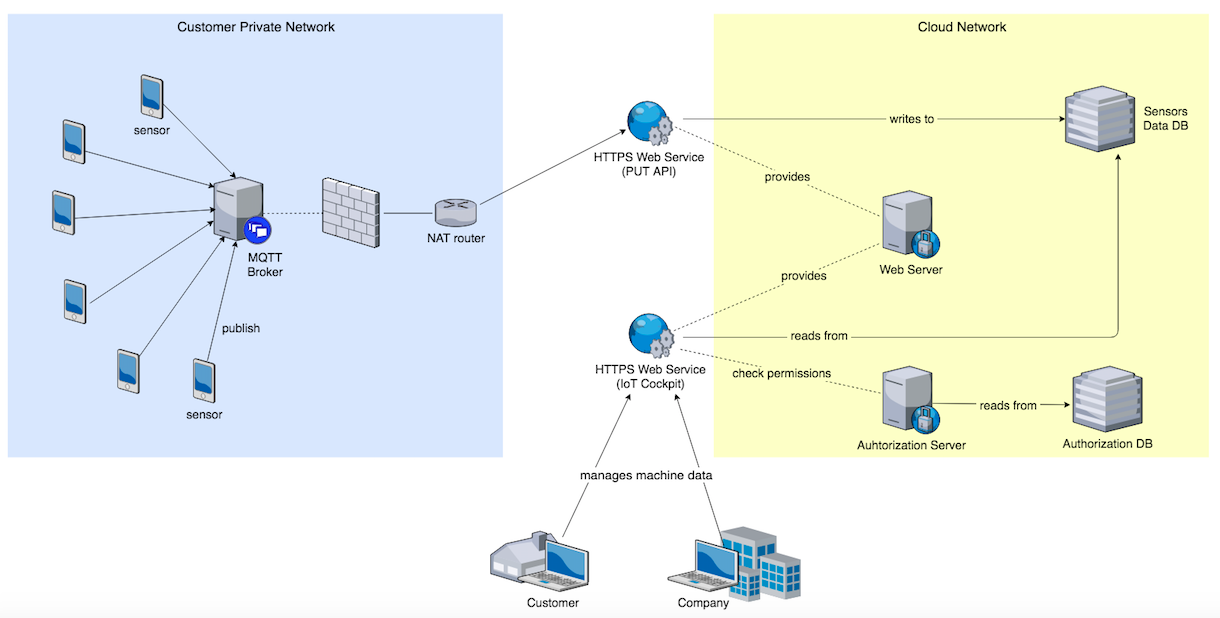
\includegraphics[width=15cm,height=11cm,keepaspectratio]{factory_architecture}
\centering
\caption{Factory Architecture}
\label{fig:factoryarchitecture}
\end{figure}

This MQTT broker is developed and provided by a third company, which is the owner of the cloud network as well as the provider of the monitoring service, and in our case we are talking about \emph{SAP}~\footnote{https://www.sap.com/}.\\
In this specific scenario, MQTT communication is not encrypted and there is no required authentication system; simply, there are several open topics, one for each sensor, which publishes its measures at regular intervals of time.\\
It is easy to understand that this is a risky choice for an industrial system architecture, that should be considered only if we can totally trust all the devices connected to the internal network.\\
Clearly, to trust all of them we have also to be sure that the internal network protection is secure enough: having a wired network defintely helps, since an attacker must have physical access, but of course this is not always possible, especially when devices belonging to the same network are not located in the same place.\\
In that case it is necessary to create a secure wireless network protected by WPA2 and a strong password.\\

As shown in Figure \ref{fig:factoryarchitecture}, the customer private network increases its security putting a firewall in front of the server hosting the MQTT broker.\\
This firewall is properly configured to hide all the devices from the external world, blocking all the incoming and outgoing connections.\\
Actually, there is only one outgoing connection allowed, that is the one that allows the server, on which the broker runs, to send the collected data by the sensors to the cloud.\\

The outgoing connection uses an \emph{HTTPS API} (simply a web service), provided by a webserver belonging to the Cloud network, so to the SAP network, whose job is to receive data from sensors and write them on the database.\\
Having to do with a secure HTTPS connection we know that data is transferred securely, therefore we can assume that the customer-side is properly protected.\\

There is just one remaining risk to be removed: only trusted clients' requests must be accepted by the \emph{PUT API}, hence those coming from the company customers' broker servers.\\
To do that, mutual authentication is employed, so when a customer's broker sends sensors' data to the API it will send also its own X.509 certificate to the remote webserver to prove its identity.\\
\underline{Note}: this is the solution chosen and implemented by SAP, but an alternative one could be to include authentication credentials in the POST content, avoiding the mutual authentication mechanism, which, as already seen, can afflict performances.
%We will discuss more in detail about this at the end of Section \ref{ssec:connectedmachines}, related to the Connected Machines architecture.

We should notice that the Factory architecture brings a great benefit in terms of certificates management: since all the customer's machines/sensors belong to the same private network and only the server is allowed to establish outgoing connections, then just one X.509 client certificate is necessary for all of them.\\

One last thing to notice is that, considering what has been said so far, it seems that the customer has no way to verify if the data sent to the API has been correctly received and stored on the Cloud.\\
This is not true, in fact the customer, as well as the company itself, can verify the health status of their machines using another secure web service, called \emph{IoT Cockpit}, provided by the same webserver.\\
This service simply provides an intuitive dashboard to the user, by which he can stay updated and check their machines and measures; the difference from the other API is that this last one can be accessed by everyone but it requires a user authentication.\\


\subsection{Connected Machines}
\label{ssec:connectedmachines}
\bigskip
This second system architecture deals with a different, and more difficult to protect, scenario.\\
In this case, there are several customer's machines located in different places, probably far from each other, therefore no common and secure network protecting them, but simply standalone machines and their related sensors.\\ 

We can see this architecture in Figure \ref{fig:connectedmachines}.

\begin{figure}[H]
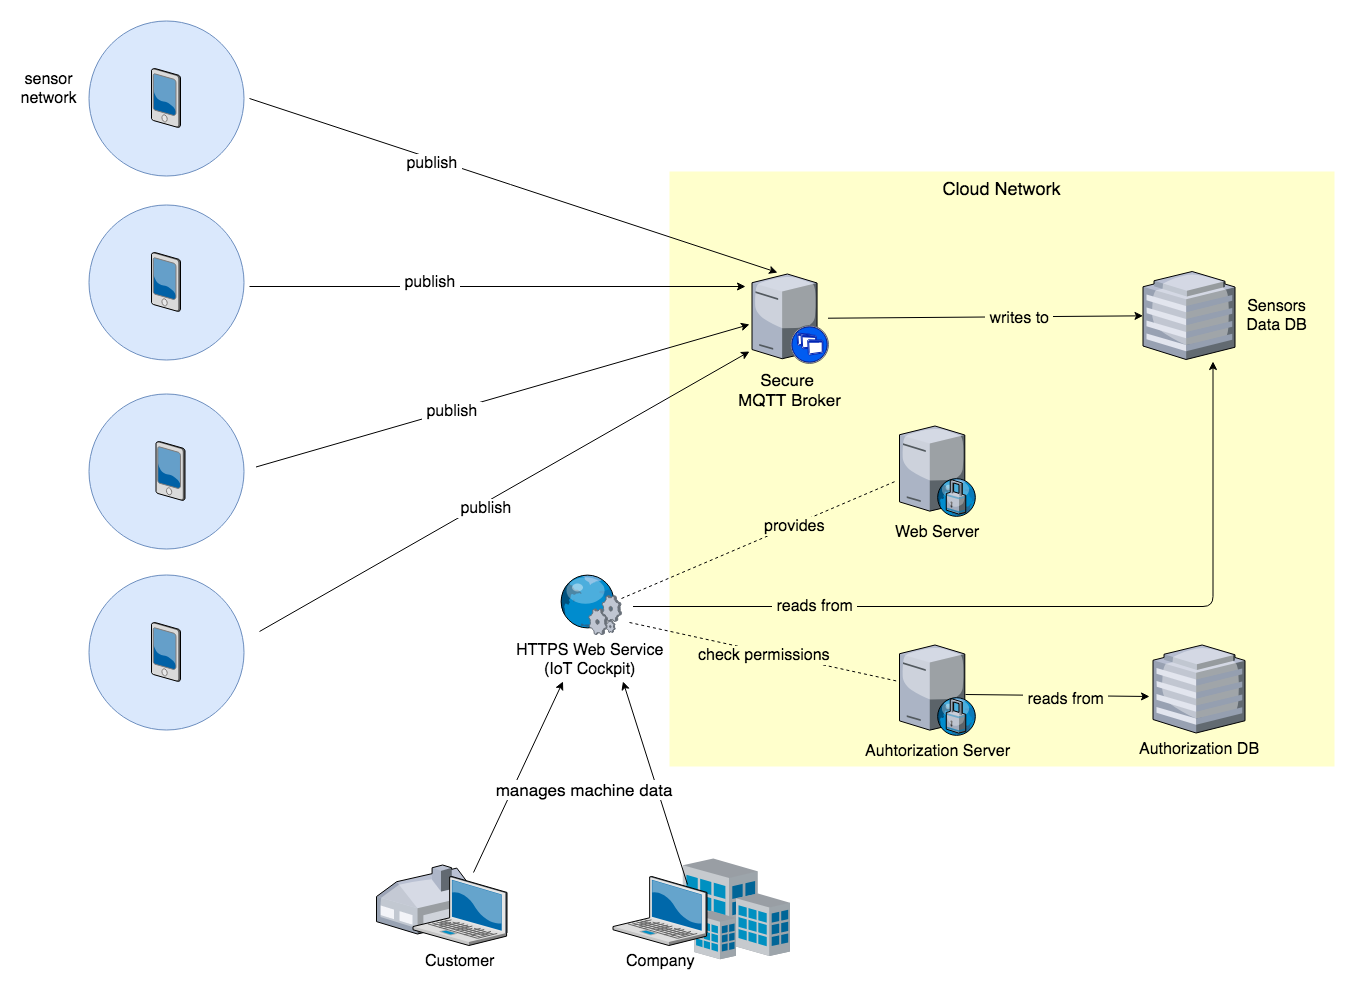
\includegraphics[width=14cm,height=11cm,keepaspectratio]{connectedmachines_architecture}
\centering
\caption{Connected Machines Architecture}
\label{fig:connectedmachines}
\end{figure}

It is obvious that this fact changes everything: it would not make sense to give each machine a local server running an MQTT broker to which send data, and then forward it to the cloud through it as before.\\
This procedure should be considered only when there are several machines close to each other which can share a private network in order to create a singular exit node towards the cloud network.\\

Having customers' sensors spread all over the world is a very common scenario; just think about sensors applied on transports, for instance sensors used to check the health status of car tires.\\

So, for all these cases there is only one way to communicate: having a remote MQTT broker on the cloud and let each sensor publishing its own data on it.\\
Clearly, this time it is necessary to use the secure version of MQTT, therefore relying on TLS.\\
As before, it is also necessary to verify if sensors' data actually come from trusted senders; we notice that in this case MQTT client authentication would be enough, but practically mutual authentication is employed again.\\

Here we have a practical example of what we have discussed before in Section \ref{sec:homemademqtt}: I recommended you to trust only certificates approved by reliable certification authorities and never trust self-signed certificates. \\
This last architecture helps us to understand that, in addition to the fact that it is not good to trust self-signed certificates, forcing the server to keep a potentially huge number of certificates is not convenient and totally pointless; therefore, the right way is to trust client's certificates which are trusted by certification authorities we trust.\\

\bigskip

After having seen these two real-world architectures, we can conclude that there is no unique perfect solution covering all cases, but it is necessary to find the most proper one for the specific scenario we are dealing with, considering all the relevant factors, such as networks topologies, performances, secrecy, integrity, users' needs, maintenance.\\



\section{Case 2 - Every aspect is important }
\bigskip
This second case is certainly less detailed than the previous one, but I would like to quickly discuss it because it helps to show how every aspect of a system should be considered important as the others, and as trivial errors can lead to serious consequences.\\

In the previous case we have seen that the monitoring system was provided by SAP; we can say that, currently, the company relies on the SAP platform for most of its projects, and SAP structure is very solid and secure, paying attention to be up to date with the newest security measures to take.\\
For more information, you can consult their official documentation at \\ \texttt{https://www.sap.com/corporate/en/company/security.html}.\\

This is a real case, but again, for obvious privacy reasons, I cannot disclose to the customer I am going to talk about.\\

In this project I had to take some real-time data, stored on a remote server belonging to the customer, and send them to another remote server through a secure MQTT channel.\\
I started Wireshark to sniff data and see if it was possible for an attacker to alter the measures, but without success as the MQTT channel used TLS.\\

What we did not say is that the protocol used to recover data from the source server was FTP, which is known to be extremely vulnerable since it sends data in plain-text.\\


So, the moral of this brief story is that it is fundamental to consider every security aspect of the system before developing it, because all the efforts involved in the successful implementation of a communication channel can be undermined by a very bad implementation of another communication channel.\\


\part{ZigBee}

\chapter{Protocol Overview}

\section{Introduction}
\bigskip

ZigBee is a low-cost protocol developed by ZigBee Alliance, for low-power wireless personal area networks that interconnect devices primarily for personal uses within a short range (10-100 meters). \\
This communication system is less expensive than Wi-Fi and it has a larger range than Bluetooth, besides its range can also be extended using routers.\\

Nowadays, ZigBee is used in industrial automation, where industries exploit it to manage and monitor critical equipments, but in particular this protocol is perfectly suited for controlling home appliances remotely. We may think to TVs, surveillance devices, locks, thermostats, lighting system, garage door, windows, blinds, speakers, as well as any other home system that can be controlled remotely.\\
Currently, ZigBee is mainly used to build \emph{Smart Homes}.\\

In section \ref{sec:zigbeearch} we start to analyze the architecture and the basic concepts of this protocol. Security issues are described in the next chapter.\\

\clearpage
\section{Architecture and basic concepts}
\label{sec:zigbeearch}
\bigskip
As we can see in Figure \ref{fig:zigbeearch}, a ZigBee system consists of three types of devices:

\begin{itemize}
\setlength{\itemindent}{+4mm}
\item[$\bullet$] \emph{Coordinator}: they manage the overall network and they are responsible for starting it, allowing other devices to join it, keeping track of them and configuring the security level of the network.\\
A coordinator is considered as the \emph{Trust Center (TC)}, which performs security control of the network, storing and distributing the  keys.\\
For all these reasons, the coordinator never sleeps, instead it must be continuously powered.


\item[$\bullet$] \emph{Routers}: they are intermediary devices responsible for routing packets between end devices or between an end device and the coordinator.\\
Routers, as well as end devices, need to be accepted in the network by the coordinator.\\
Routers have two things in common with the coordinator: 1) they cannot sleep, 2) they can give permissions to new devices to join the network.

\item[$\bullet$] \emph{End devices}: they are low-power, or battery-power, devices (usually sensors) that can communicate only through their parent nodes.\\
Unlike routers, end devices cannot route traffic and they can go to sleep to reduce power consumption.
\end{itemize}

\begin{figure}[H]
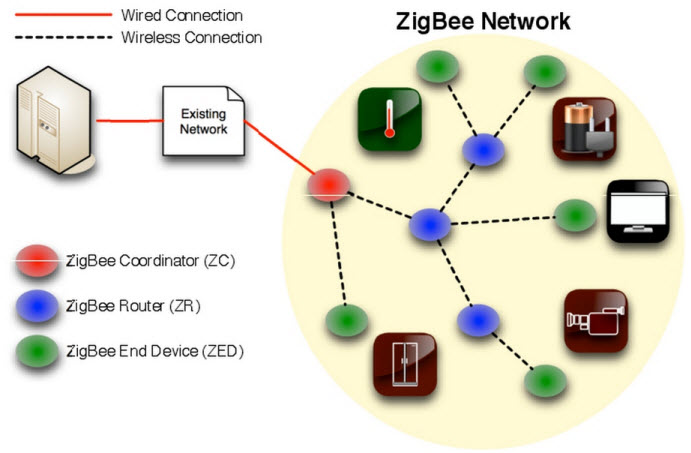
\includegraphics[width=12cm,height=12cm,keepaspectratio]{zigbee_architecture}
\centering
\caption{ZigBee Architecture}
\label{fig:zigbeearch}
\end{figure}

There is no required number of specific components for a ZigBee network, instead the number of coordinators, routers and devices depends on the network we want to build and its topology (\emph{star, cluster tree or mesh}).

\subsection{ZigBee network topologies}
\bigskip
Figure \ref{fig:zigbeetopologies} shows the three possible ZigBee network topologies: star, tree and mesh.

\begin{figure}[H]
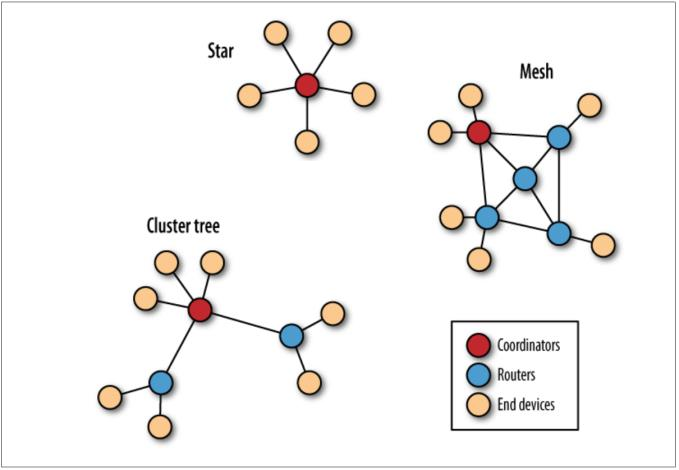
\includegraphics[width=11cm,height=11cm,keepaspectratio]{zigbee_topologies}
\centering
\caption{ZigBee Topologies}
\label{fig:zigbeetopologies}
\end{figure}

\begin{itemize}
\setlength{\itemindent}{+4mm}
\item[$\bullet$] \emph{Star}: in this topology there is only the coordinator responsible for initiating and managing the network devices; since every device talks directly with the coordinator, we consider the other devices as end devices, therefore no routers in this topology.\\
This topology is mainly used when all the endpoints need to communicate with a central controller, so it is common in industries.\\
Of course this topology is very simple, but its simplicity is also its greatest weakness, in fact the coordinator is a single point of failure, because if it breaks down the whole network goes down.

\item[$\bullet$] \emph{Tree}: this topology has a root node, represented by the coordinator, which is responsible for establishing the network and choosing the proper key network parameters.\\
This time we have even routers, which can have either the coordinator or another router as parent node, and they are responsible for routing data packets through the network using hierarchical routing strategy.\\
This solution is not so better than the previous one because we still have a single point of failure, given by the coordinator, besides children nodes become unreachable if their parent node breaks down.

\item[$\bullet$] \emph{Mesh}: this topology has, as usual, a single coordinator, several routers to extend the network and, of course, end devices.\\
Once again, the coordinator establishes the network and is responsible to choose the network parameters.\\
There is no more a single point of failure because in this case we have multiple paths to reach a node, therefore a more robust protection from link failures.\\
The only drawback of this topology is that is complex and more difficult to set up than the previous ones.\\
\end{itemize}

Mesh topologies are more robust than the others, therefore they are the most used.\\

\clearpage
\subsection{Protocol Stack}
\bigskip

The protocol is based on the IEEE 802.15.4 standard, which provides the physical and MAC layers, while the above layers are given by ZigBee.\\
Each layer provides a set of services exposed to the upper layer.

\begin{figure}[H]
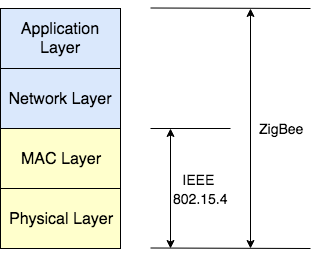
\includegraphics[width=6cm,height=6cm,keepaspectratio]{zigbee_stack}
\centering
\caption{ZigBee Protocol Stack}
\end{figure}

Let us briefly see them: 

\begin{itemize}
\setlength{\itemindent}{+4mm}
\item[$\bullet$] \emph{Physical Layer}: it provides the basic radio communication capabilities, such as channels, modulation, demodulation, transmission rate, etc.
\item[$\bullet$] \emph{Medium Access Control layer (MAC)}: it manages data transmissions between neighbor devices (point to point). 
It includes services like transmission retry and acknowledgment management~\cite{digi}.
\item[$\bullet$] \emph{Network Layer}: it adds routing capabilities that allows data packets to traverse multiple devices (multiple hops) to route data from source to destination, in order to create more complex topologies.
\item[$\bullet$] \emph{Application Layer}: it provides device and service discovery features, applications supporting layer primitives used by devices, capabilities to manage the security policies and configuration of a device. Finally, it collaborates with the Network layer to establish and manage cryptographic keys, and provides primitives for their management.

\iffalse
it consists of ZigBee device objects (ZDOs), Application support sub-layer (APS) and the Application Framework, where: 
 
\begin{itemize}
\item \emph{ZDOs} are applications supporting layer primitives used by end devices, routers and coordinators.\\ 
Furthermore, ZDOs manages the security policies and configuration of a device.
\item \emph{APS} provides a communication bridge between the Network Layer and the Application Layer, collaborating with the network layer to establish and managing cryptographic keys, and provides primitives for the management of cryptographic keys to the upper layers.
\item \emph{Application Framework} is nothing but the environment in which application objects are hosted.\\

\end{itemize}
\fi
\end{itemize}

\subsection{ZigBee communication modes}
\bigskip
ZigBee employs two communication modes:
\bigskip
\begin{itemize}
\setlength{\itemindent}{+4mm}
\item[$\bullet$] \emph{Beacon}: the coordinator periodically sends a beacon message to the devices and these wait for it before sending messages addressed to the coordinator, as you can see in Figure \ref{fig:zigbeebeaconmode}.\\
When the transmission is completed, the coordinator set a schedule for the next beacon so that the device can go to sleep till that moment.\\
Beacon intervals can be from 15 ms up to 252 seconds.\\
In this mode, all the devices know when to communicate with the coordinator.\\
Beacon mode is mainly used when the coordinator runs on batteries, hence it needs to save as much power as possible.

\begin{figure}[H]
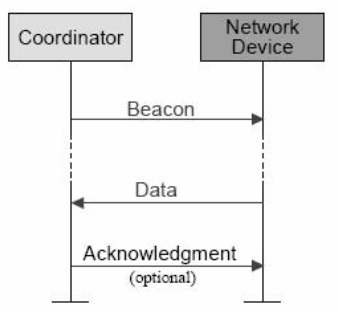
\includegraphics[width=7cm,height=7cm,keepaspectratio]{zigbee_beaconmode}
\centering
\caption{Beacon mode}
\label{fig:zigbeebeaconmode}
\end{figure}

\item[$\bullet$] \emph{Non-Beacon}: in this case the coordinator is mains-powered and wait continuously for data from the devices, which can transmit at random intervals.\\
This mode is used in systems where devices are almost always 'asleep' (for instance, in smoke detector systems).\\
Clearly, it might happen that an end device finds the channel busy and in that case the coordinator will miss the call.

\begin{figure}[H]
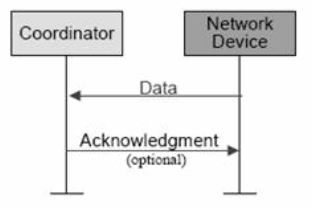
\includegraphics[width=7cm,height=7.5cm,keepaspectratio]{zigbee_nonbeaconmode}
\centering
\caption{Non-Beacon mode}
\end{figure}

\end{itemize}
\bigskip
%In chapter \ref{chap:zigbeesecchap} we start to discuss the security aspects of this protocol.\\

\chapter{Security Overview}
\label{chap:zigbeesecchap}

\section{Introduction}
\bigskip
As already said in the MQTT part, IoT will play a primary role in the coming years and for this reason it is fundamental to take care about its security.\\
While MQTT security is mainly aimed to help companies and industries to transfer their production data reliably, ZigBee has more to do with personal area networks that interconnect devices primarily for personal uses, hence high personalized and sensitive data.\\
Just think to a smart home based on ZigBee: a lot of user sensitive information can be leaked by an attacker if the security aspect is neglected.\\
Data theft is not the only problem, in fact an attacker would cause a lot of problems to the user if he could control his household appliances.\\
Just think about a thief, good enough to find and exploit a ZigBee vulnerability and turn off the surveillance devices.\\\\

In the next sections, we are going to discuss the security measures offered and adopted by the ZigBee standard; more in details, we will analyze its security models, keys (types, generation and management), authentication mechanisms and protection from some famous attacks.\\


\clearpage
\section{Security assumptions}
\label{sec:zigbeesecassumptions}
\bigskip
Being ZigBee a simple as well as low-cost communication protocol, it relies on a symmetric-key cryptography to protect network messages and devices, precisely AES 128 bits, avoiding heavier encryption system, like the asymmetric one; therefore, both the sender and recipient of a protected transaction need to share the same key.\\

All the ZigBee security features we discuss are strictly related to the cryptographic (symmetric) keys used by the protocol; in order to talk about them, we must first take a look at the following list of assumptions~\cite{secanalysisofzigbee} on which they are based:

\begin{itemize}
\setlength{\itemindent}{+4mm}
%\item[$\bullet$] \emph{ZigBee employes an open-trust model}, which means that the stack layers trust each other, therefore the layer that originates a frame must secure it
\item[$\bullet$] communication between different stack layers on the same device is not encrypted
\item[$\bullet$] cryptographic keys are securely stored in tamper proof hardware devices
\item[$\bullet$] keys are always transmitted encrypted, so never revealed
\item[$\bullet$] cryptographic mechanism and security policies are properly implemented
\item[$\bullet$] availability of almost perfect random number generators\\
\end{itemize}

\clearpage
\section{Security models}
\bigskip

ZigBee provides two network security architectures, or models, visible in Figure \ref{fig:zigbeemodels}: \emph{centralized} and \emph{distributed}.\\

\begin{figure}[H]
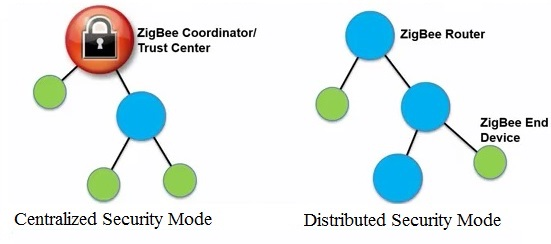
\includegraphics[width=10cm,height=10cm,keepaspectratio]{security_models}
\centering
\caption{ZigBee Security Models}
\label{fig:zigbeemodels}
\end{figure}

The difference between them concerns only the way they accept new joining devices into the network and how messages are protected.\\

Each network has a key used to encrypt broadcast messages, called \emph{network key}, and a key shared by any two devices to communicate, as well as to encrypt and provide the network key, called \emph{link key}.\\

The idea of the \emph{distributed security model} is pretty simple: there is no coordinator, but only routers and end devices.\\
In this model, we totally rely on routers to accept new routers and end devices within the network as well as to generate and distribute network keys.\\

This security model expects all the devices to share the same network key and to be pre-configured with the same link key that will be used to send the encrypted message containing the network key.\\
All the devices will talk to each other encrypting messages with the same network key, therefore everyone accepted within the network can read everyone else's data.\\

The \emph{centralized security model} is a bit more complex, but even more secure.\\
In this case we have routers, end devices and the coordinator, that from now on we will call \emph{Trust Center (TC)}.\\
This time the responsible for the management and acceptance of routers and end devices joining the network as well as the creation and sharing of the keys is the TC.\\
Besides, devices have not to be all pre-configured with the same link key and they have not to communicate with each other using the network key to encrypt messages.\\
The TC also creates and provides a new network key periodically, in order to protect the network from possible attackers, who can try to steal it.\\

While the first model is certainly simpler it is less secure, and almost unused, so we focus on the second one}.\\

{\setlength{\parindent}{0cm}
We have already mentioned that a ZigBee network exploits two main types of keys to communicate securely: \emph{network keys} and \emph{link keys}.\\
}
%Actually, there is also a third key, called \emph{master key}.\\
Let us see them in details:

\begin{itemize}
\setlength{\itemindent}{+4mm}
\item[$\bullet$] the \emph{network key} is a 128-bit key generated and distributed by the TC to all the network devices in order to allow them to communicate in broadcast securely.\\
It is clear that the TC cannot send the network key in plain-text, otherwise an attacker could sniff that, making it useless. Sending a key without encrypting the message is against one of the assumptions we have seen in section \ref{sec:zigbeesecassumptions}, but unfortunately there is one exceptional case in which this happens.\\

There are two types of network keys, \emph{standard} and \emph{high security}, which differ from each other in the way they are distributed to joining devices. \\
A high-security network key is sent encrypted, while the other one in plain-text.\\
More specifically, the standard network key is sent in plain in those cases where the end device that wants to join the network has no pre-configured link key. Some TCs decide to deny the access to such devices, while others are more permissive and allow them to join the network, risking to compromise the security of the whole network.\\

It is important to notice that joining devices can be also pre-configured with a network key, but this is a uncommon practice, since, as already said,  in a centralized model the network key is updated periodically by the TC.
\item[$\bullet$] the \emph{link key} is a 128-bit key shared by two devices, so between the TC and another node, or between two nodes.\\
More in details, we have three different types of link key~\cite{secanalysisofzigbee}:

\begin{itemize}
\item \emph{Pre-configured Global Link key}: it exists for one reason only, that is encrypting the network key in order to transfer it securely from the TC to the end devices.\\
As the words \emph{global} and \emph{pre-configured} suggest, this key is the same for all the network nodes and pre-installed in the devices that want to join the network.\\
The global link key can be defined by the manufacturer, or, even much simpler, by ZigBee.
\item \emph{Pre-configured Unique Link key}: same use of the previous one, but different for every node.
\item \emph{Trust Center Link Key (TCLK)}: like the last one, this key is used to allow the TC and another node to communicate securely, but the difference is that this time it is not pre-configured.\\
The TC generates it randomly or derive it from the network key (or from the pre-configured unique link key, if existent) using an hash function.\\ 
Without entering in too many details about this hash function, we just say that it takes two 128-bit keys as input and return one 128-bit key as output; the second input key of the function is known only by the TC.\\
Of course, this generated key must be sent to the interested node, and to do that the TC uses once again the network key or, much better, the pre-configured unique link key, if existent.\\

A reasonable question is \emph{``why should we generate a TCLK if we already have a pre-configured link key?"}; I did not find a specific answer to this question, but I guess that the reason is that, being the pre-configured link key rarely updated, changing the link key we use to communicate and avoiding to use our pre-configured link key helps us to protect it and give less chance to an attacker to steal it.
\item \emph{Application Link Key}: similar to the previous one, but used by pairs of nodes.\\
The generation and provisioning of the key is quite intuitive: one of the two devices requests the key to the TC, which is responsible to generate and send it to both of them using their respective pre-configured unique link key or, if not existent, the network key.
\end{itemize}

\iffalse
\item[$\bullet$] the \emph{master key}:  This is a shared key used, during the execution of a symmetric-key key establishment protocol (\emph{SKKE}), to generate link keys~\cite{zigbeespec}.\\
Without going into too much detail, if a initiator device and a responder device share the master key, they can use it to establish a link key following these three basic steps:

\begin{enumerate}
\item the exchange of ephemeral data
\item the use of this ephemeral data to derive the link key
\item the confirmation that this link key was correctly computed
\end{enumerate}
This key provisioning way is almost never used, so we focus only on the two previous ones.
\fi

\end{itemize}

Now that we have analyzed the ZigBee security keys and their provisioning, I would like to report, just for completeness, that there exists a (rarely used) extension of the traditional key-transport, which involves certificates.\\
Security keys can be distributed using the \emph{Certificate-Based Key Establishment protocol (CBKE)}~\cite{zigbeesecbasics2}, which implements a mechanism to allow devices to negotiate symmetric unique keys with the TC, starting from a certificate, signed by a Certification Authority, that both devices must have.\\
The CBKE mechanism allows the device to start communicating, but even the Trust Center to securely identify it.\\
The key establishment procedure involves the following four steps:

\begin{enumerate}
\setlength{\itemindent}{+5mm}
\item Exchange static data for certificate validation
\item Generate the key
\item Derive a MAC (\emph{Message Authentication Code}) key
\item Confirm the key using the MAC
 \end{enumerate}

The key generation and the MAC derivation use the \emph{Elliptic Curve MQV}\footnote{https://www.ecmqv.com/} and a key derivation function.\\
At the end of this process, both the Trust Center and the device \emph{i} share a new Link Key LK\textsubscript{i}, which is used to encrypt the TCLK they are going to use to communicate.\\
Now, if two devices \emph{i} and \emph{j} have obtained their TC Link Key, and want to communicate with each other, they can obtain their Application Link key by asking it to the TC, as usual, which will generate a random Application Link Key LK\textsubscript{ij} and send it to both the devices using their respective Trust Center Link Key.\\

\iffalse
\subsection{Over-The-Air Updates}
\bigskip
We have already mentioned that in a centralized architecture the TC periodically updates and distributes the network key in order not to give attackers time to try to steal it.\\
Clearly, the updates of the network key are sent over-the-air, so they must be encrypted with some keys, which usually are either the current network key or the TC Link key (unique or global, depending on the scenario).\\
Obviously, the second one is a better and more secure choice, because if an attacker has already stolen the current network key, and the TC uses such key to encrypt the new one, then the attacker can always obtain the updated network key.\\
%Let's clarify that each node is able to store several network keys, but also to identify the current one with a unique key sequence number assigned by the Trust Center.\\

Keys are not the only things we may think to update over the air, in fact ZigBee gives the user the chance to update a device, adding new features as well as applying security patches, if necessary.\\
Clearly, if this kind of communication is not protected enough, it might happen that devices accept some critical fake updates from untrusted sources.\\
Assuming, for instance, we want to send an updated code image to a device to apply a security patch, we firstly sign the image with a private key k\textsubscript{1}, then we send the image over the network using a second cipher key k\textsubscript{2}; doing this only the end device will be able to decrypt it and verify the validity of the image thanks to its tag (it is clear that the end device must know the two keys used to encrypt and create the tag).\\
Once the device received the message, it decrypts and validates it, then updates itself.\\
\fi

\clearpage
\section{Protocol Stack Security}
\bigskip
In this section we discuss the security measures adopted by the ZigBee protocol stack, which involves the MAC, Network and Application layers.\\

The IEEE MAC Layer implements security services which are used by the ZigBee protocol in the network and application layers.\\ 
IEEE 802.15.4 establishes the encryption algorithm to use (AES) when the data has to be transmitted, but the standard does not specify the keys or security levels to use.
This is a task concerning the upper layers, hence ZigBee is responsible for that.

\subsection{802.15.4 Security}
\bigskip

\subsubsection{Security Control Header}
\bigskip
Let's start taking a look at Figure \ref{fig:zigbeemacframestruc}, representing the structure of a MAC data frame~\cite{security802154}.\\

\begin{figure}[H]
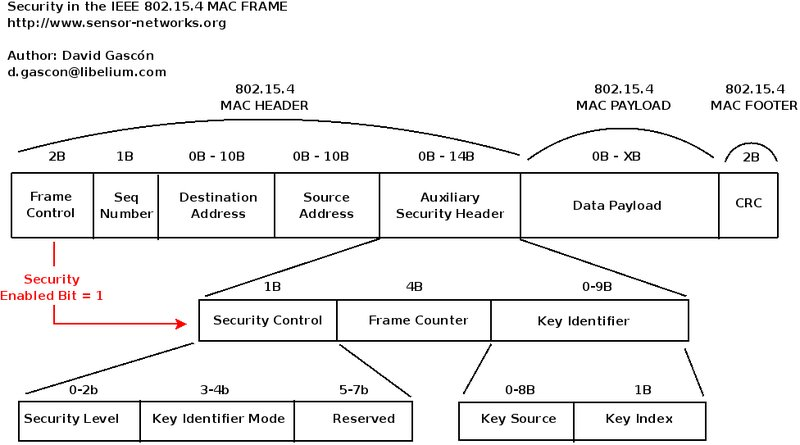
\includegraphics[width=13cm,height=13cm,keepaspectratio]{mac_frame}
\centering
\caption{ZigBee MAC Frame's Structure}
\label{fig:zigbeemacframestruc}
\end{figure}

IEEE 802.15.4 MAC frames contain a specific header dedicated to security, called \emph{Auxiliary Security Header}.\\
This header is enabled only if the \emph{Security Enabled} bit, contained in the \emph{Frame Control} field, is set to 1.\\
There are three subfields inside the Auxiliary Security Header:

\begin{itemize}
\setlength{\itemindent}{+4mm}
\item[$\bullet$] \emph{Security Control}: it is used to specify the type of protection provided by the network.\\
The most important subfield of the Security Control field is \emph{Security Level}, which can assume eight different values, each of them providing a different degree of encryption and integrity checks, and is the place where our global security policy is set.

\begin{center}
\small
   \begin{tabular}{ | c | c | c | c |}
    \hline
    Security Level & Security Attributes & Data Encryption & Integrity Check \\ \hline
    0x00 & None & N & N \\ \hline
    0x01 & AES-CBC-MAC-32 & N & Y\\ \hline
    0x02 & AES-CBC-MAC-64 & N & Y \\ \hline
    0x03 & AES-CBC-MAC-128 & N & Y\\ \hline
    0x04 & AES-CTR & Y & N\\ \hline
    0x05 & AES-CCM-32 & Y & Y\\ \hline
    0x06 & AES-CCM-64 & Y & Y\\ \hline
    0x07 & AES-CCM-128 & Y &Y\\ \hline
    \end{tabular}
\end{center}

\iffalse
\begin{figure}[H]
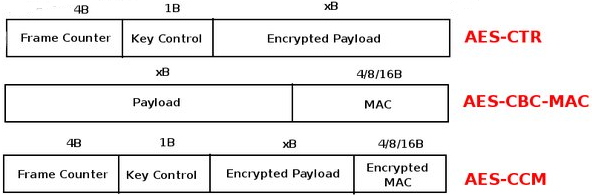
\includegraphics[width=10cm,height=9cm,keepaspectratio]{datapayload_fields}
\centering
\caption{Data Payload possible configurations}
\end{figure}
\fi

\begin{itemize}
\setlength{\itemindent}{+4mm}
\item \emph{AES-CTR}: data payload is encrypted using AES 128-bit counter mode.
\item \emph{AES-CBC-MAC}: data payload is not encrypted, but a Message Authentication Code (MAC) is computed and attached to the end of the   data payload.\\
The MAC is created encrypting information from the 802.15.4 header and the data payload.
Its length can be 32 bits, 64 bits, or 128 bits, depending on the specified security level, but in any case it is calculated using a 128 bit key.
\item \emph{AES-CCM}: it is the combination of the two previous ones.\\
More details about this algorithm will be discussed in section \ref{ssec:zigbeesecfeatures}.
\end{itemize}

\item[$\bullet$] \emph{Frame Counter}: it is a simple counter given by the source of the current frame in order to protect the message from replay attacks. 

\item[$\bullet$] \emph{Key Identifier}: it contains useful information to know which key we are using with the node we are communicating with.\\
\end{itemize}

\subsubsection{Access Control List (ACL)}
\bigskip

Each 802.15.4 device can have an \emph{Access Control List (ACL)}, which is a list containing the so-called \emph{``trusted-brothers"} and their respective security policies.\\
More in details, for each trusted brother we store the following information:

\begin{itemize}
\setlength{\itemindent}{+4mm}
\item[$\bullet$] \emph{Address}: the physical address of the node we want to communicate with
\item[$\bullet$] \emph{Security suite}: the encryption algorithm to use (\emph{AES-CTR}, \emph{AES-CCM-32}, etc)
\item[$\bullet$] \emph{Key}: the 128-bit key used in the AES algorithm
\item[$\bullet$] \emph{Last Initial Vector (IV)/ Frame Counter}: this is an incremental value used 1) by the source to encrypt the message and 2) by the recipient as frame counter to avoid replay attacks.\\
\end{itemize}

In simple words, when a node wants to communicate with another node (send or receive a message) it looks at the ACL to see if it is a trusted brother; in that case it uses the security measures contained in the respective security policy.\\\\

\subsection{ZigBee Security features}
\label{ssec:zigbeesecfeatures}
\bigskip
The ZigBee security architecture includes security mechanisms, such as frame protection, at three layers of the protocol stack: MAC, Network and Application.\\
Each layer is responsible for its own security processing but, as already said, the keys and the security level used by the MAC Layer are established by the upper layers.
%They set the default key of the MAC Layer equal to the current network key and its link keys equal to the current link keys of the upper layers.

\subsubsection{Frame Protection}
\bigskip
In addition to the security features provided by IEEE 802.15.4 standard, Zigbee adopts \emph{AES CCM*} to protect network and application layers frames.\\
As for the MAC layer, frames have an Auxiliary Security Header and a payload field, which can be encrypted and contain a MAC for data integrity.\\
Figure \ref{fig:zigbeenwkframestruc} and \ref{fig:zigbeeapsframestruc} show you the structure of these two frames.\\

\begin{figure}[H]
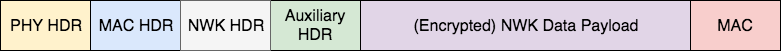
\includegraphics[width=13cm,height=11cm,keepaspectratio]{nwk_frame}
\centering
\caption{ZigBee NWK Frame's Structure}
\label{fig:zigbeenwkframestruc}
\end{figure}

\begin{figure}[H]
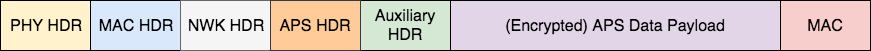
\includegraphics[width=13cm,height=13cm,keepaspectratio]{aps_frame}
\centering
\caption{ZigBee APL Frame's Structure}
\label{fig:zigbeeapsframestruc}
\end{figure}


\emph{CCM mode} combines \emph{CBC-MAC} and \emph{CTR}: CBC-MAC is used to generate a tag for the frame, and CTR is used to encrypt the frame itself as well as the generated tag.\\
\emph{CCM* mode} is nothing but a minor variation of CCM, which includes all the features of CCM and, in addition to them, it offers encryption-only and integrity-only capabilities.\\
Using AES-CCM* is convenient because it can cover all the security levels provided by the 802.15.4 standard, simply turning on, or off, the integrity-only and the encryption-only capability.\\

Clearly, the receiver uses AES-CCM* and the proper key to decrypt the encrypted frame and the tag, then he generates the MAC on his own in order to compare it with the received one.\\
The key used to encrypt and generate the MAC for a frame, is the one specified in the receiver's ACL; ZigBee simplify the protocol security, using the same key for all the layers.\\


\subsubsection{Replay Attacks Protection}
\bigskip
We have already mentioned that ZigBee offers protection from replay attacks, using a frame counter.\\
More in details, every node in the network has a 32-bit frame counter which is incremented at every packet transmission.\\
Besides, each device tracks the previous frame counter of every node with which it has communicated because, doing this, if a node receives a packet from another node with the same or lesser frame counter value than it had previously received, the packet will be dropped.\\
It is important to say that the frame counter is reset to 0 when the Trust Center updates the network key.

\subsubsection{Device Authentication}
\bigskip
Clearly, only authorized and authenticated devices can join the network.\\
The Trust Center is responsible to accept new devices that want to join the network, but before doing that the device must be able to receive a network key and set proper attributes within a limited given time to be considered authenticated.\\
More in details, there are two different procedures for authenticating devices:

\begin{itemize}
\setlength{\itemindent}{+4mm}
\item[$\bullet$] \emph{Standard (Residential) mode}: if the new joining device already has a pre-configured network key (unlikely), it will receive an all-zero network key from the trust center as part of the authentication procedure.\\
If the new device does not have a network key and not even a link key (which must be known by the Trust Center obviously), the TC  sends the network key in plain, which is a quite important vulnerability.\\
Since the new device does not know the address of the trust center, it will use the source address of the received message to set the trust center address.

\item[$\bullet$] \emph{High Security (Commercial) mode}: in this second, and more secure, mode the Trust Center never sends the network key over an unprotected communication channel.\\
If the device has a valid pre-configured link key, global or unique, to communicate with the TC, then this last one will send the network key to it, and will consider it as authenticated.\\
A global link key requires less memory to the Trust Center, but it is less secure than the unique link key.\\
Instead, if no pre-configured link key is owned by the device, then the Trust Center expects it to have, at least, the master key by which it is possible to start the key establishment protocol, after that the device and the TC will share the link key.\\
The new device has a limited time to complete the key establishment, otherwise it has to leave the network and retry the authentication procedure again.\\
When and if the link key is confirmed, the Trust Center considers the device as authenticated for commercial mode, and can send the network key to it through a secure channel thanks to the just established link key.\\

This second mode seems to be more secure than the previous one, and surely it is, but it actually has a vulnerability: if the new device does not share a master key with the Trust Center, this last one will send it over an unprotected link. 

\end{itemize}

\subsubsection{Network Interference Protection}
\bigskip
It might happen that nearby wireless networks, even Wi-Fi or other ones, create physical interferences to our ZigBee network.\\
Without entering in too many details, it is important to know that ZigBee and IEEE 802.15.4 try to reduce the presence of interferences using low RF transmission power, low duty cycle and the CSMA/CA mechanism.\\
Often, this is not enough, so ZigBee provides two other strategies to avoid interferences:

\begin{itemize}
\setlength{\itemindent}{+4mm}
\item[$\bullet$] \emph{Collaborative}: ZigBee network and other networks work together; in simple words, when one network is active, the other one remains inactive in order to avoid packet collisions.\\
Clearly, this method expects the two networks to share a communication channel to manage the collaboration.

\item[$\bullet$] \emph{Non-Collaborative}: in this second method, ZigBee network has no communication channel shared with nearby wireless networks, but it uses several interferences detection techniques to avoid as many interferences as possible.\\
We will not discuss the following techniques, since they are outside the context, but for completeness I will provide a list of some of them:

\begin{itemize}
\setlength{\itemindent}{+4mm}
\item \emph{CSMA/CA}
\item \emph{Signal spreading-spreading methods}
\item \emph{Frequency Channel selection}
\item \emph{Adaptive Packet Length Selection}\\
\end{itemize}

\end{itemize}


We conclude this section saying that ZigBee takes care about security, as we have understood so far discussing its security measures.\\
But we have also seen some important vulnerabilities in the exchange of keys, that, just right now, makes the protocol not perfect at all.\\
This is not surprising since ZigBee was designed to keep devices low-cost and low-energy.\\

%In section \ref{sec:zigbeevulns} we will discuss the most relevant ZigBee vulnerabilities.


\clearpage
\section{ZigBee vulnerabilities}
\label{sec:zigbeevulns}
\bigskip
The aim of this section is to discuss the most relevant ZigBee vulnerabilities and some practical attacks to exploit a ZigBee network.\\
Some of them are related to the specific implementation, while some others are strictly related to the protocol itself.\\
Let's see each of them in details:

\begin{itemize}
\setlength{\itemindent}{+4mm}
\item[$\bullet$] \emph{Key storage}: previously, we mentioned that ZigBee assumes that keys are securely stored within the devices, but this is not always the case.\\
If an attacker can extract the network key from a device, then all the communications within the network will be at risk.

\item[$\bullet$] \emph{Key transportation}: if the Trust Center operates in residential mode, it could happen that the network key is sent in plain; clearly, this is a quite important vulnerability since we transmit the key shared by all the devices within the network to send broadcast messages with no protection at all, compromising the whole network.

\item[$\bullet$] \emph{Ghost Attack}: frame counter checks allow recipient devices to ignore duplicate messages, but a \emph{Denial of Service (DoS)} vulnerability persists: if an attacker captures an authentic message and replay it, the recipient will discard it but it will spend time and energy to check its validity.\\
If an attacker performs tons of replay attacks against the same target, the battery life of this last one will be drastically reduced (especially considering that we are talking about low-power devices).

\iffalse
\item[$\bullet$] \emph{Predictable sensor polling rates}: as we know, end devices can put themselves in sleep mode and wake up at regular intervals to poll the coordinator for data inputs or, in beacon mode, when it receives a beacon from the coordinator, in order to save their battery-life.\\
This mechanism gives the attacker an advantage: it can send crafted messages to a device at regular intervals even if it is not necessary, forcing it to wake up and process the received messages.\\
Switching from sleep mode to active mode requires a rather big amount of energy, as well as processing invalid messages, as we have just seen.\\
So, this is nothing but an extension of the previous Ghost Attack, which has been proved to be extremely effective.
\fi

\item[$\bullet$] \emph{Manufacturer-defined Link Keys}: manufacturers set default link keys within their devices, and sometimes these keys are used to join ZigBee networks.\\
Using manufacturer default link keys is a bad choice, because they are usually publicly available.

\item[$\bullet$] \emph{Association Flooding}: by default, there is no integrity checks on acknowledgment packets, therefore an attacker can send fake ACKs to devices, and they will be considered as authentic.\\
An attacker, within an already compromised network, can keep on reading messages sent by a device even if the respective recipient is not responding, simply sending fake ACK packets to the sender every time it sniffs a message from it. 

\item[$\bullet$] \emph{No protection from DoS attacks}: ZigBee has no known denial of service protection mechanisms.\\
There are several ways to perform a DoS attack against a device:


\begin{itemize}
\setlength{\itemindent}{+4mm}
\item \emph{Set the frame counter to its maximum value}: an attacker can send a frame to other devices setting the frame counter to the largest acceptable value and spoofing its address pretending to be another device of the network.\\
This last one can no longer communicate with the other devices as it is impossibile to create a valid frame counter.
This is the simplest DoS attack, but fortunately it is possible only in those situations where there is no integrity check on the frame.

\item \emph{Flooding}: it consists in simply sending tons of messages towards victim devices. For instance, an attacker could replay all the messages it is able to capture (or create legit messages, if it already knows the network key).\\
This kind of attack where the replay messages are sent to all the network devices is called \emph{broadcast storm attack}.

\item \emph{Physical Jamming}: this is a physical attack which involves tools able to cause signal interferences big enough to prevent communication among devices.

%\item \emph{Sinkhole attack}: this attack consists in sending messages in the network in order to compromise communication, altering the routing tables and redirecting the traffic to a fake device through fake routing paths, which cannot be able to carry on the transmission.
\end{itemize}

\item[$\bullet$] \emph{No key re-using control}: a device is allowed to join the network using the same link key several times (even forever if no explicit constraint is specified), but this is a poor choice because if an attacker is good enough to steal the link key of the device, then it will be able to spoof the authentic device credentials and join the network pretending to be it.

\item[$\bullet$] \emph{Trap networks}: since a ZigBee device tries to connect directly to the first available network (or probably the one with the strongest signal) without asking anything to the user, then an attacker could create a fake network which would work as a kind of trap for the device.

\item[$\bullet$] \emph{Statistical attacks}: an attacker can obtain several information about the functioning of a ZigBee network if it analyzes its traffic properly using statistical algorithms.\\ 
\end{itemize}

\clearpage
\section{Considerations and best practices}
\bigskip
We conclude this second and last part about ZigBee by listing some considerations:

\begin{itemize}
\setlength{\itemindent}{+4mm}
\item[$\bullet$] the protocol itself is not much secure, regardless of its implementation
\item[$\bullet$] the protocol works well if all the devices within the considered network can protect themselves from keys theft
%\item[$\bullet$] choose carefully the physical devices based on the role they will have within the network. For instance 
\item[$\bullet$] always enable frame encryption to protect frame content, but especially to guarantee their integrity
\item[$\bullet$] it would be better to always use the commercial mode, which is more secure than the standard one (even if not much secure anyway)
\item[$\bullet$] avoid using manufacturer link keys, and remember that they are often public
\item[$\bullet$] prefer unique keys rather than global ones every time you can
\item[$\bullet$] it is recommended to test your network with a dedicated security tool, like \emph{Killerbee}\footnote{https://github.com/riverloopsec/killerbee}, before deploying it (especially in productive scenarios)
\item[$\bullet$] you can specify the list of authorized devices, using the Trust Center's Access Control List, and specify the devices with which each device can communicate using its own ACL.
%\item[$\bullet$] consider the addition of spoofing detection techniques, if possible
\item[$\bullet$] it is not recommended to use ZigBee in places covered by many wireless networks because interferences are difficult to remove and communication's quality will be poor.
\item[$\bullet$] select the frequency band that generates the least interference with other wireless systems.\\
\end{itemize}

The considerations above should help you to understand how to build an almost secure and reliable ZigBee network, but I would like to clarify a last thing, which is probably even more important than the previous ones.\\
ZigBee was born almost fifteen years ago when devices had much less computational power than today and they needed a very light-weight and low power-consumption protocol to be able to communicate with each other.\\Besides, despite the protocol was designed with security in mind, there are still too many protocol's features that inevitably lead to relevant security risks.\\
In addition to security problems, there are also many communication malfunctions such as possible interferences with other wireless networks, loss of key synchronization, loss of periodic key updates.\\

Nowadays, technological progress is surprisingly fast, and even very small devices often have enough computational power and battery-life to support \emph{Wi-Fi} protocol, which is more secure, reliable, easier to configure and continuously improved.\\
I conclude this section, saying that, in my opinion, ZigBee is a not so secure protocol having many security problems, which should be considered only if treating with extremely constrained devices, otherwise choosing other more modern and efficient protocols, such as Wi-Fi, is a better choice.\\

\chapter{Conclusion}

After having discussed the main theoretical security concepts of these two important IoT protocols, I would like to conclude my thesis making some considerations about their current importance and business reality usage.\\

In 1999 MQTT was developed as a lightweight messaging protocol to enable low-energy monitoring of an oil pipeline. Nowadays it is considered as the most efficient protocol for IoT devices and was adopted as an international standard for IoT by \emph{OASIS}.\\

More and more people and companies show interest in MQTT, as confirmed by \emph{Google Trends}, which highlights a strong and continuously growing interest related to the keyword ``MQTT" in the recent years, as we can see in Figure \ref{fig:mqtt_googletrends}.

\begin{figure}[H]
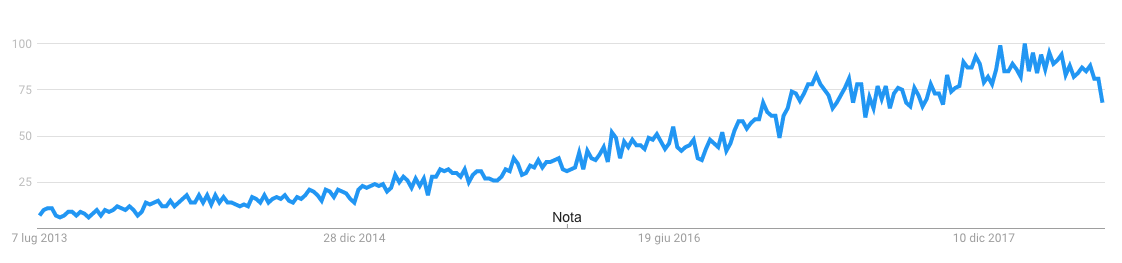
\includegraphics[width=14cm,height=12.5cm,keepaspectratio]{mqtt_googletrends}
\centering
\caption{MQTT - Google Trends Statistics}
\label{fig:mqtt_googletrends}
\end{figure}

Previously, we have seen in Figure \ref{fig:shodanres} a relevant number of active MQTT servers obtained using Shodan.\\
Being it a rapidly growing number, I decided to draw a graph better representing the number of active MQTT servers I found day by day in the last two weeks.\\
Figure \ref{fig:activeserversgraph} shows us the obtained result.

\begin{figure}[H]
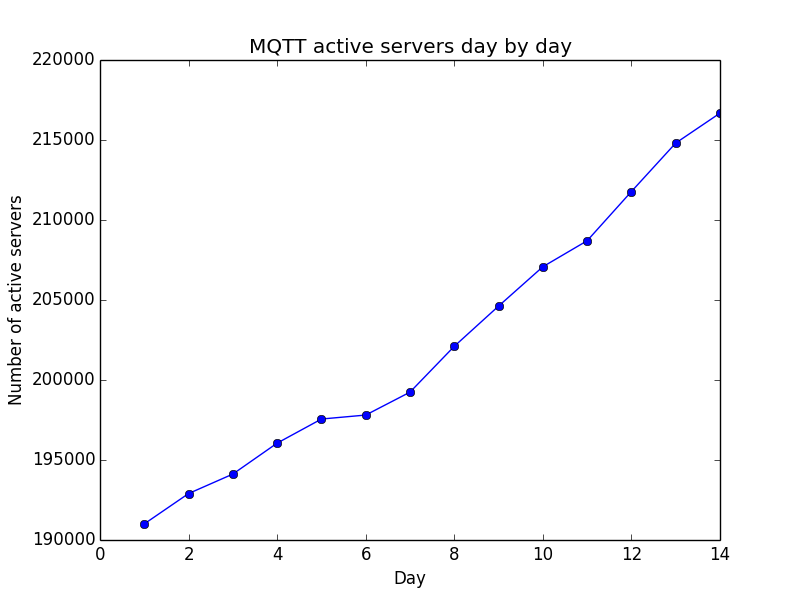
\includegraphics[width=12cm,height=10cm,keepaspectratio]{conteggio_servers_grafico}
\centering
\caption{MQTT daily active servers}
\label{fig:activeserversgraph}
\end{figure}

I would have also liked to draw a graph representing the number of insecure servers over time, but unfortunately for doing so it is necessary to pay a fairly expensive Shodan API key.\\
Anyway, considering what we have said so far, I guess that the graph would be very similar to this last one.\\\\

MQTT meets all of IoT's needs, in fact it is specialized in connecting low-bandwidth devices having limited CPUs, bringing a very little overhead, with a central hub. Just think about the huge number of systems involving energy monitoring sensors pushing communication to a remote monitoring location for analysis.\\

Due to its simplicity and efficiency, MQTT is adaptable to a wide variety of applications in different industries. Even ABO DATA uses this protocol for most of its applications.\\
Furthermore, making secure MQTT communication is pretty simple thanks to the TLS support, but despite this, during my internship I learned that there are so many aspects to consider before making secure and reliable applications, such as customers' needs and deadlines.\\

The main reason why many MQTT systems are not secure is that customers are not interested or not even aware about security issues.\\
Besides deadlines must be respected, and what I have personally seen is that customers are much more interested to working applications rather than secure ones, hence most of times the first goal is to simply complete the task without considering security issues.\\\\

Talking about ZigBee, Figure \ref{fig:zigbee_googletrends} shows us that the interest in this protocol has almost remained constant in the recent years.

\begin{figure}[H]
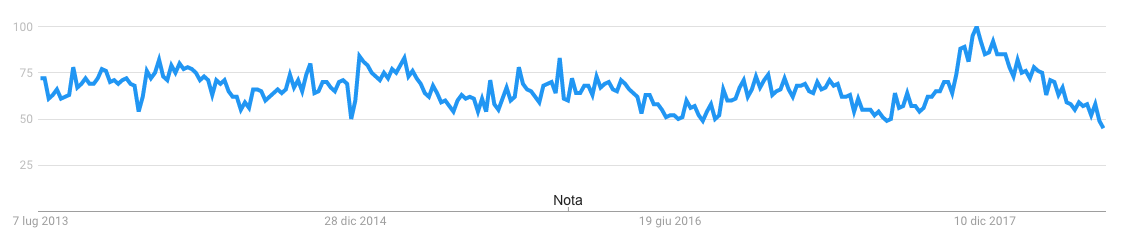
\includegraphics[width=14cm,height=12.5cm,keepaspectratio]{zigbee_googletrends}
\centering
\caption{ZigBee - Google Trends Statistics}
\label{fig:zigbee_googletrends}
\end{figure}

ZigBee, similar to MQTT, is primarily designed for very constrained devices, having an even lower overhead, thanks to its low-rate communication.\\
The relevant differences between them are the standards on which they are built, the security measures (e.g. ZigBee cannot simply rely on TLS as MQTT does), the possible applications and the efficiency as well as the reliability.\\

Unfortunately, I have not had the opportunity to work with this protocol during my internship, so all I know is what I have read or heard from external sources.\\

What I think about this protocol is that it is still not considered as important and revolutionary as MQTT, because it is mainly suited for smart home applications and domotic, which are interesting applications but currently still not much in vogue and necessary.\\ Besides, this protocol has many security vulnerabilities and communication problems (e.g. missing network key transports/updates, many hard-to-remove physical interferences).\\
Finally, since technology is growing extremely fast, even small devices are becoming more and more powerful and able to support other heavier wireless protocols, like Wi-Fi, which is definitely much more widespread.\\
Moreover, researchers are being to bring down power requirements of Wi-Fi based systems, so that they can perform at low energy levels like ZigBee does.\\




\bibliography{tesiref} 
\bibliographystyle{unsrt}



\end{document}





















